

\newpage
\clearpage
\pagenumbering{roman}
\tableofcontents



\clearpage
\pagenumbering{arabic}

%%New section means new page
\newcommand{\sectionbreak}{\clearpage}

\section{Introduction}


%Joachim Start
\subsection{MOS Transistor Structure}


    \subsubsection{MIS}  Metal-Insulator-Semiconductor, consists of a conductor and a semiconductor, separated by thin insulation layer.
    \subsubsection{MOS}  Metal-Oxide-Silicon, a version of MIS, in which silicon dioxide ($SiO_2$) is used as oxide.
    \subsubsection{CMOS}  Complementary Metal Oxide Silicon, a MOS process in which both nFET and pFET are fabricated on the same substrate.
    \subsubsection{MOSFET} Metal-Oxide-Semiconductor Field-Effect Transistor, built using MOS and a p-n junction diode.
    


\begin{figure}[htbp]
  \centering
  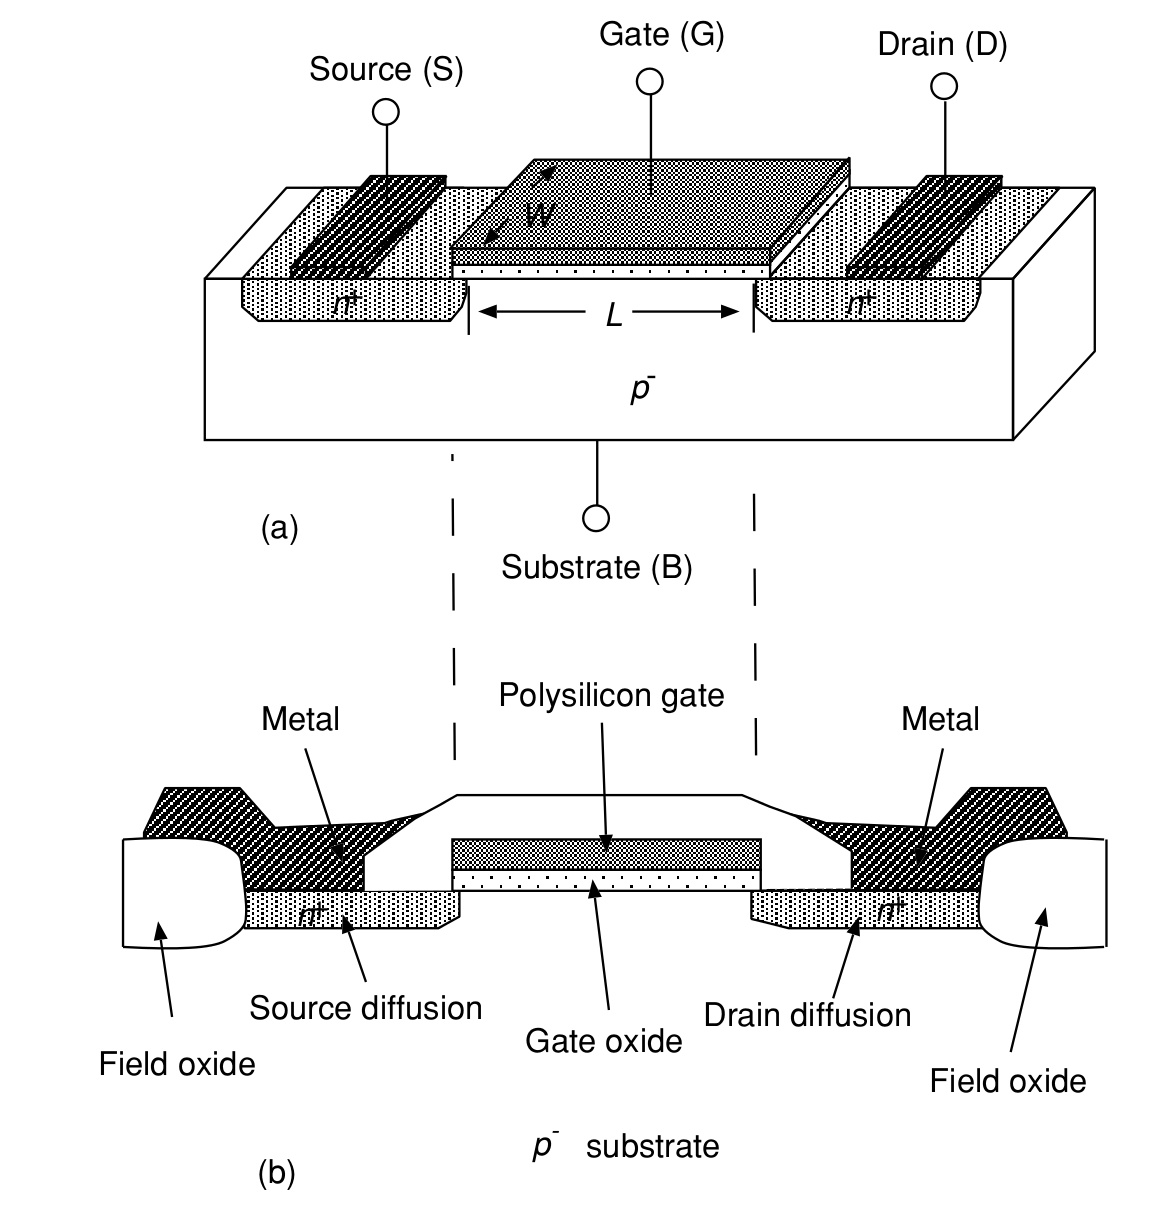
\includegraphics[scale=0.8]{pics/MOSFET_Structure.jpg}
  \caption{Structure of an n-type MOSFET in a pbody. The MOSFET has four terminals; the drain (D), the source (S), the gate (G), and the bulk (B). (a) Pictorial view of the MOSFET. (b) A more realistic picture of a cross-section of a fabricated MOSFET. Note that the gate oxide is much thinner than the field oxide. \cite{book:VLSI}}
  \label{fig:MOSFET_Structure}
\end{figure}\bigskip

\bigskip\subsection{MOS Transistor Terminals}
We can view the transistor as having four terminals:
\begin{enumerate}
\item Gate (G)
\item Source (S)
\item Drain (D)
\item Bulk (B)
\end{enumerate}

\bigskip\subsection{MOS Transistor Types}
\subsubsection{n-type}
    Because the n+ source and drain regions can supply a lot of electrons to the channel, this device is called an n-channel MOSFET (nFET,n-type MOSFET, NMOS) \cite{book:VLSI}
\subsubsection{p-type}
   In p-channel MOSFET (pFET,p-type MOSFET, PMOS) , the charge in the channel is carried by holes supplied from the source and drain regions.
    
\bigskip\subsection{MOS Transistor in Substrate}
Most CMOS processes use a p-type starting substrate.  The nFETs rest in the common $p^-$ substrate, and the pFETs rest in
n-wells within the substrate as shown in Fig. \ref{fig:MOSFET_Physical_Structure}

\begin{figure}[htbp]
  \centering
  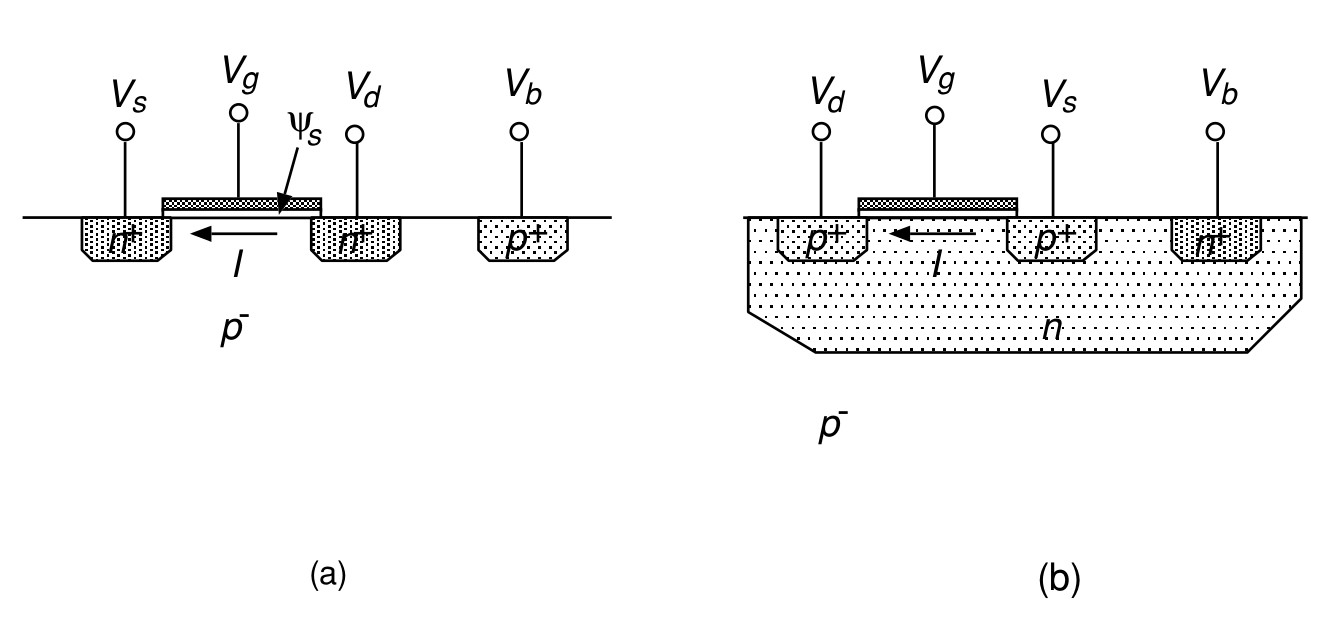
\includegraphics[scale=0.8]{pics/MOSFET_Physical_structure.jpg}
  \caption{Physical structure of (a) an nFET and (b) a pFET in a common $p^-$ substrate. The pFET rests in a n-well within the substrate. \cite{book:VLSI}}
  \label{fig:MOSFET_Physical_Structure}
\end{figure}

\bigskip\subsection{MOS Transistor Biasing}
\subsubsection{nFET}
To ensure only a small leakage current between the $n^+$ regions to the p-substrate, the junctions have to be reverse biased.
To do this, the drain voltage $V_d$ and the source voltage $V_s$ of the nFET should be greater than or equal to the bulk voltage $V_b$:
\begin{equation}
V_{sb}=V_s-V_b \geq 0
\end{equation}
\begin{equation}
V_{db}=V_d-V_b \geq 0
\end{equation}

The location of drain and source is defined by the carrier flow:\cite{book:VLSI}
\begin{itemize}
\item Electrons are supplied to the channel by the source, and removed by the drain.
\item Holes are supplied to the channel by the source, and removed by the drain.

\end{itemize}

The $n^+$ region biased at the higher voltage is called the drain, and the other $n^+$ region is called the source. Because electrons are negatively charged, the direction of positive current flow,
I, is from drain to source, even though the carriers flow from source to drain. \cite{book:VLSI}

\subsubsection{pFET}
In pFET , the $p^+$ regions should be biased negative relative to the bulk to reverse-bias the pn junctions.
\begin{equation}
V_{sb} \leq 0
\end{equation}
\begin{equation}
V_{db} \leq 0
\end{equation}

\subsection{MOS Transistor Channel}
The region underneath the gate and between the source and drain regions is called the channel. The channel has a width W, and a length L
. The channel is insulated from the gate above by a layer of silicon dioxide. The gate is made of heavily doped (low resistivity) polycrystalline silicon.
\cite{book:VLSI}

\subsection{MIS Operation Domains}
Depending on the charge of the gate, we either attract or repel majority carriers on the surface of the channel semiconductor.\\
\textbf{Important: }Relevant here is the type of substrate (p or n) the channel is made of, don't confuse it with nFET or pFET!
\begin{figure}[H]
  \centering
  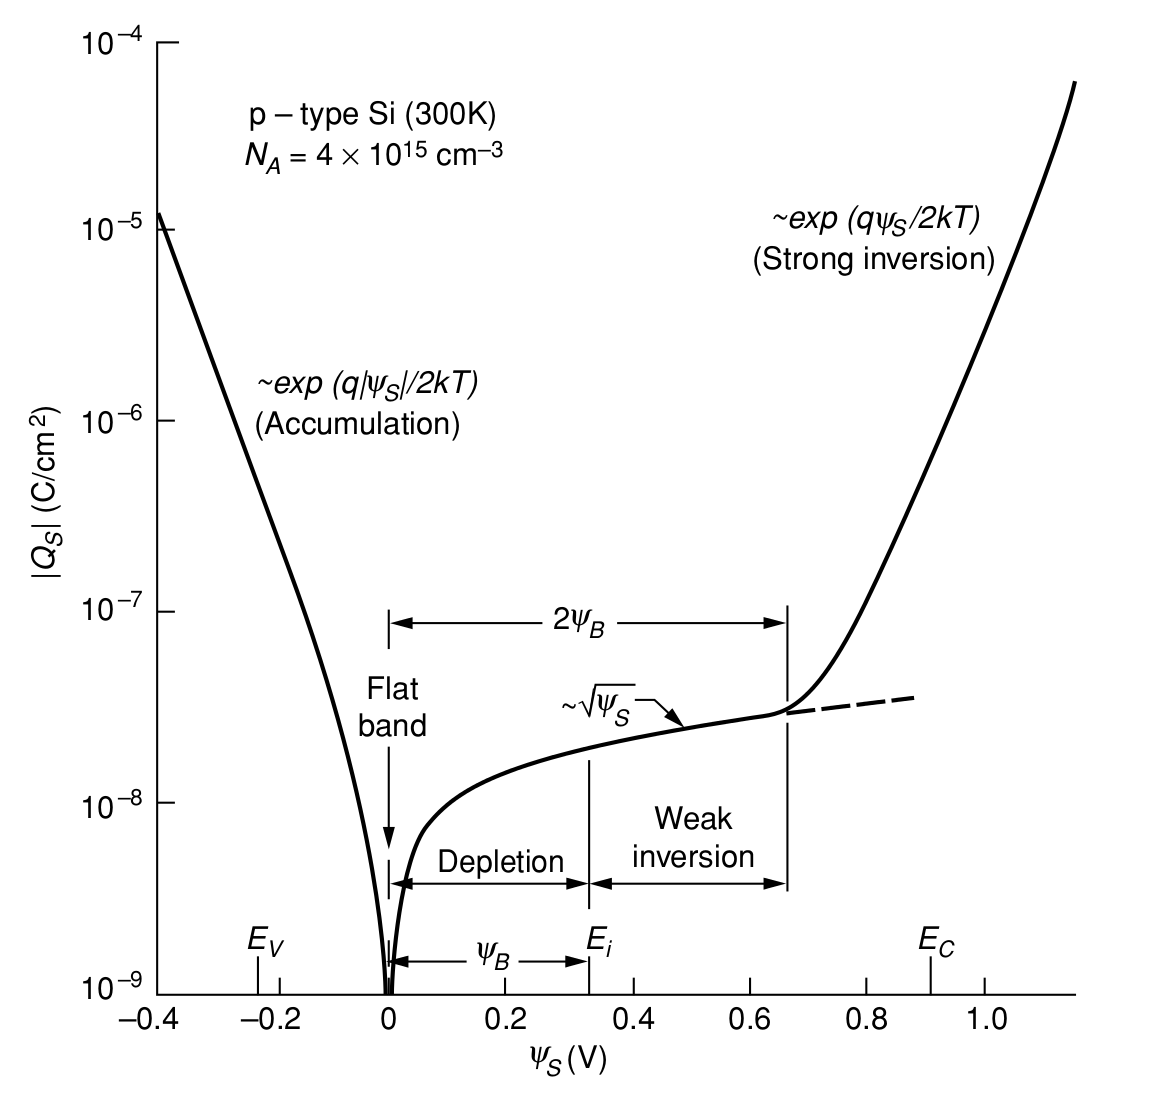
\includegraphics[scale=1]{pics/operation_domains.png}
  \caption{Dependence of the area charge $Q_s$ on the surface potential for p-type silicon with acceptor density $N_A = 4 \times 10^15cm^-3$ at room temperature. Figure adapted from S. M. Sze (1981), Physics of
Semiconductor Devices, 2nd Edition. \copyright 1981 by John Wiley $\&$ Sons, Inc.  \cite{book:VLSI}}
  \label{fig:coperation_domains}
\end{figure}



\subsubsection{Accumulated Transistor Channel}
Accumulation happens when a charge on the gate attracts a lot of majority carriers on the surface of the semiconductor underneath it.\\
For a p-substrate channel (default), as shown in figure \ref{fig:channel_accumulated}, a negative voltage on the gate means mobile electrons on the gate. These electrons (negatively charged) attract positive charges on the semiconductor surface underneath it, leading to accumulation of them. Since positive charges (holes) are the majority carrier in p-substrate, we call this situation accumulation.\\\\
In a n-substrate channel, positive charge on the gate leads to accumulation of electrons (majority carriers in n-substrate) on the channel surface.
\begin{figure}[H]
  \centering
  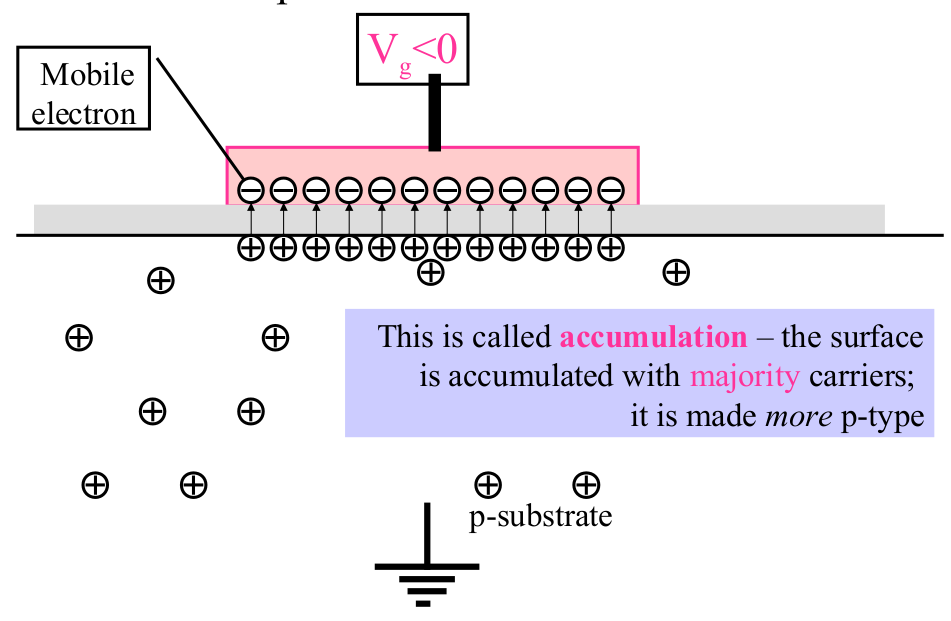
\includegraphics[scale=1]{pics/channel_accumulation.png}
  \caption{Accumulated Transistor Channel \cite{lec2}}
  \label{fig:channel_accumulated}
\end{figure}


\subsubsection{Flat-Band Transistor Channel}
In an ideal MIS diode, with no bias applied, the work function of the metal and the semiconductor are the same.  The Fermi levels line up and the energy bands in the semiconductor are flat. $\rightarrow$ Flat-Band Condition \cite{book:VLSI}\\
With $V_g=V_{fb}=0$, the majority carrier density is constant and equal to the dopant density.
\begin{figure}[H]
  \centering
  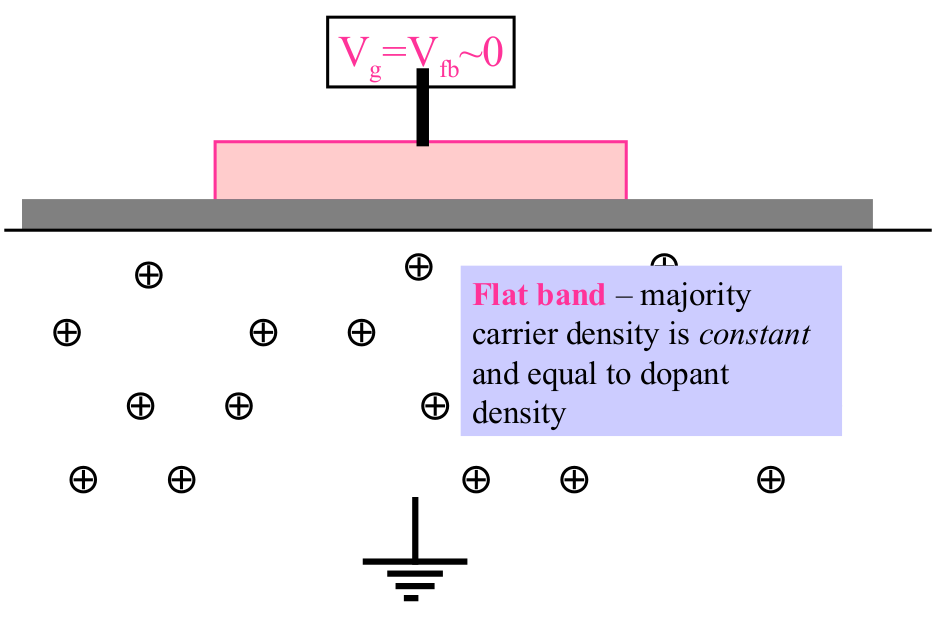
\includegraphics[scale=1]{pics/channel_flat_band.png}
  \caption{Flat-Band Transistor Channel \cite{lec2}}
  \label{fig:channel_flat_band}
\end{figure}

\subsubsection{Depleted Transistor Channel}

For a p-substrate channel, if we put a positive subthreshold voltage on the gate (positive charges), we repulse positive majority carriers on the semiconductor surface. $\rightarrow$ Depletion of majority carriers.\\
For a n-substrate channel, the same happens if we put a subthreshold negative charge on the gate. $\rightarrow$ Depletion of electrons (majority carrier in n substrate) on the semiconductor surface.

\begin{figure}[H]
  \centering
  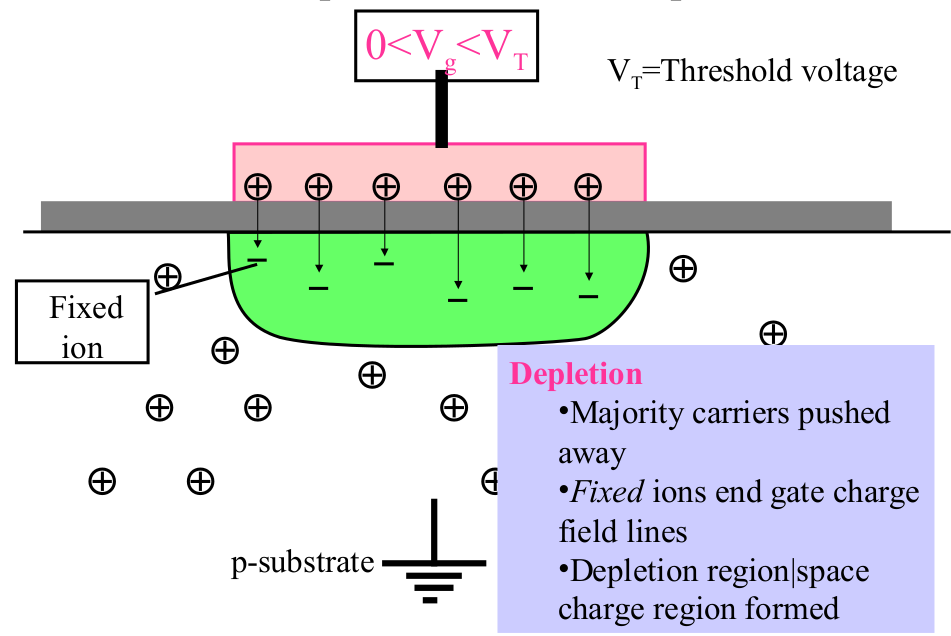
\includegraphics[scale=1]{pics/channel_depletion.png}
  \caption{Depleted Transistor Channel \cite{lec2}}
  \label{fig:channel_depletion}
\end{figure}

\subsubsection{Inverted Transistor Channel}
For a depleted p-substrate channel, if we now further increse the postive charge on the gate, we will reach a point where we start attracting negative minority carriers on the semiconductor surface. The surface becomes inverted. (p-type $\rightarrow$ n-type and vice versa in n substrate)  $\rightarrow$ Inversion
\begin{figure}[H]
  \centering
  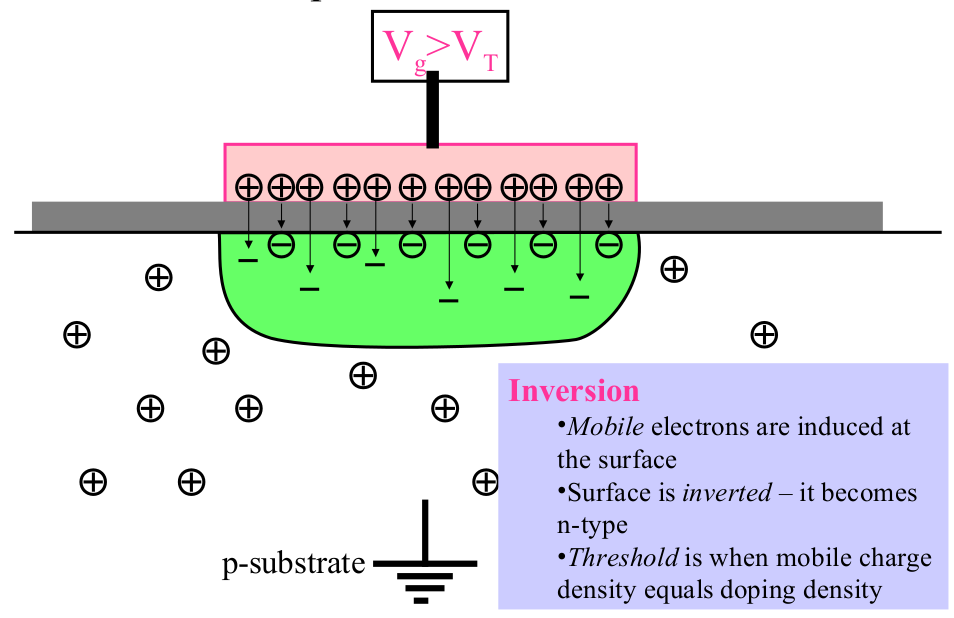
\includegraphics[scale=1]{pics/channel_inversion.png}
  \caption{Inverted Transistor Channel \cite{lec2}}
  \label{fig:channel_inversion}
\end{figure}

%Joachim End



\section{On capacitance, MOSFETs, and regions}
%David
We start with nomenclature. There are two basic kinds of MOSFETs\footnote{Metal-Oxide-Semiconductor [what it's made of] Field Effect Transistor [how it works]}: nFETs and pFETs. These are sometimes also called $n$-channel and $p$-channel transistors (respectively), and – in an $n$-well device – native and well transistors (respectively). The nFET has an $n$-type source and drain sitting in a $p$-type substrate, and the pFET is vice-versa.\\ \\
We have devices now – things to plug in. You tie the nFET's drain to a higher voltage than its \textsl{source} (which will \textsl{source} electrons), and the pFET is vice-versa (because it will \textsl{source} holes). ``Source'' and ``drain'' are so named because they respectively \textsl{source} and \textsl{drain} the majority mobile carrier of the given transistor type.\\ \\
You don't want current crossing the $pn$ junctions where the drain and source sit in the substrate, so we reverse bias those junctions\footnote{Put $n$ at a higher voltage than $p$}. That means we stick the nFET bulk to ground (usually hardwired on the chip), and keep $V_s, V_d > 0$. Look at that – we've plugged it in! \\ \\
We know about the sub- and above threshold regions. Moving between these two regions is a function of $V_g$, specifically the voltage between the gate and the source ($V_{gs} = V_g - V_s$). Both the sub- and the above threshold regions are divided into the triode\footnote{Interesting but irrelevant: ``triode'' comes from the original thought behind the transistor as a 3-terminal diode, thus \emph{tri-}ode vs. \emph{di}-ode. The entire transistor history on Wikipedia is a really interesting read.} and saturation regimes. For both sides of the threshold, we move in and out of saturation by changing $V_{ds}$ – the drain-source voltage.\\ \\
\textsl{This is important: changing \emph{gate-source} voltage from low to high moves us from subthreshold to above threshold for \emph{any} $V_{ds} > 0$. Similarly, changing \emph{drain-source} voltage from low to high moves us from ohmic regime to saturation regime for \emph{any} $V_{gs} > 0$.} \\ \\
Surface voltage $\psi_s$ deserves another mention. We've built a transistor, plugged it in, and biased the gate relative to the bulk\footnote{Really, we care about all voltages \emph{relative to the bulk}, but bulk is almost always at ground so it's an implicit relation}. Because of the positive gate voltage, the depletion region does not only surround the drain and source, but also extends between them. Having this channel of depletion region means that there is a built-in voltage across it\footnote{Not across it as in a \emph{drain-source} voltage, but across it as in perpendicular to the plane of the insulating oxide}. So here we have two voltages in series – one across the insulating oxide, one across the depletion region. Current isn't flowing across either of these gradients, so what does that mean? It means static, accumulated charges are hanging out on either side of the gradients. In other words: they are capacitances. The relationship between the capacitances is described by $\kappa$, which we call the \textsl{capacitive coupling ratio} from gate to channel. It describes how effectively a change in gate voltage can change the surface voltage.
%------Transistor cross-section-------
\begin{figure}[hb]
 \centering
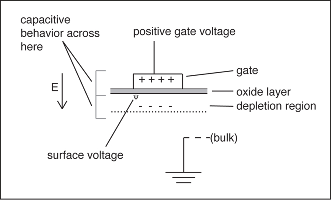
\includegraphics[natwidth=663,natheight=400]{pics/nme_xSection.pdf}
\caption{Cross-section of the transistor gate, oxide layer, and depletion region. When $V_{gate-bulk} > 0$, both the oxide insulator and the depletion region (channel) act as capacitors. See Figure 2.18, p.42 in the textbook for a proper version of this figure.\label{crossSectionCaps}}
\end{figure}
%-----------------------------------------------
%-----------------------------------------------

%Joachim
\subsection{MOSFET Operation Domains}
The operation domain of an nFET is set by the relative values of the four terminals of the transistor.\\
In general, these operation domains (e.g. accumulation) are equivalent to the ones of the MIS structure.\\
We can map the regimes to a MOSFET mode:


\begin{longtable}{ |p{4cm}|p{4cm}|p{4cm}| }
\hline
\textbf{When the MOSFET is in this domain:} & \textbf{We say the MOSFET operates in:} & \textbf{Which can be further divided into (depending on $V_{gs}$:} \\ \hline
\endhead
Accumulation & Cutoff & \\ \hline
Depletion & Cutoff & \\ \hline

Weak Inversion & Subthreshold & Triode Mode \par Saturation Mode\\ \hline
 Strong Inversion & Above Threshold & Triode Mode \par Saturation Mode\\ \hline
\end{longtable}





%David:
\section{Subthreshold behavior}
Depending on how we want a transistor to behave, we will want to keep it in subthreshold. A few of the biggest reasons to do so are low power consumption (nano- or microamps), less dominant Early voltage effects, and the usefulness of logarithmic behavior (can cover many orders of magnitude of current for less than one order of magnitude of voltage). Most circuits in this class involve subthreshold transistors, so these are extremely important concepts to understand. In this chapter I will discuss only nFET transistors. To do the equations for pFET devices, you simply multiply all voltages by $-1$\footnote{We did not previously mention this, but pFET bulks are tied to $V_{dd}$, not ground, so all voltages are relative to that (that is, the relevant $V_{g}$ for a pFET would be calculated as $V_{dd} - V_{g}$). The same goes for drain and source voltages. Generally, what the bulk is tied to is hard-wired into the device, though sometimes we make a device where there is a fourth lead controlling this.}.
%-----------------------------------------------
\subsection{On subs, threshes, and holds}
Yeah it's a bad section title. Don't worry about it. We mentioned $\kappa$ above. It's pretty darn important, so let's look at the mathematical definition:
\begin{equation}
\kappa = \frac{C_{ox}}{C_{ox} + C_{dep}} = \frac{\partial\psi_s}{\partial V_g}
\label{kappaEqn}
\end{equation}
where $C_{ox}$ is the capacitance across the insulating oxide and $C_{dep}$ is the capacitance across the depletion layer, as illustrated in Figure~\ref{crossSectionCaps}. $\psi_s$ is a function of a number of terms, but this is what it boils down to and why it is important\footnote{p.44 in the textbook has details on how the partial derivative comes into play, but the lecture slides do a better job of making this point}. Typical values for $\kappa$ are between 0.4 and 0.9, though it clearly must - mathematically - be less than 1 (look at ~\eqref{kappaEqn}) \\ \\
%-------MOSFET circuit diagram--------
\begin{figure}[ht]
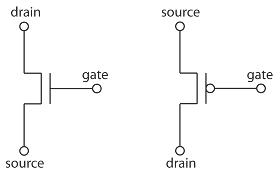
\includegraphics[natwidth=560,natheight=350]{pics/nme_mosfets.pdf}
\caption{Circuit diagrams for an nFET (left) and a pFET (right). Terminals are labeled such that, in a standard circuit diagram, $V_{dd}$ is above the components and $ground$ is below them. However, nothing in the device forces it to be this way. They are physically symmetric and can work with current flowing in either direction. \label{mosfetsFig}}
\end{figure}
%-------------------------------------
Okay, so we're subthreshold. $V_{gs}$ is low but non-zero. Let's say the source and drain, both of which are $n$-type material sitting in the $p$-type substrate, are also both at $0V$ relative to ground. Because of the low gate voltage, the electrons have an energy barrier to overcome\footnote{That's not the best way to put it. The built-in potential from the $pn$ junctions creates the energy barrier. This voltage will be such that the $n$-type material (drain and source in an nFET) is at a higher voltage than the $p$-type material (the substrate in an nFET), so due to the electric field electrons want to flow from $p$-type to $n$. If we then increase $V_g$, the positive charge on the gate pushes the \emph{substrate's} mobile carriers (holes) away from the silicon oxide, leaving a negatively-charged depletion region immediately under the surface. This is the channel where we see inversion - this is how we form the inversion layer. Broadening this channel (increasing $V_g$) makes it take less energy for an electron to move from the drain or source into the channel, and \emph{that} is what's happening with the energy barrier.} if they want to travel between drain or source and the channel. It's difficult - the natural state is quite resistive. Raising the gate voltage (but keeping it under 0.7V, the approximate threshold voltage) means electrons can more easily move through the channel because the energy barrier is lower. But they have no reason to move. It is not more favorable energy-wise to be at the source compared to being at the drain, because drain-source voltage is still zero.\\ \\
We raise the drain voltage, though only a little. Tens of millivolts. The drain side now has a slightly higher energy barrier for its electrons to cross if they want to enter the channel\footnote{This energy barrier stuff takes a little thinking to get used to, but soon you don't worry about this because you only care about the ``what,'' not the ``why.'' They spend a reasonable amount of time on it in class, so pay attention and ask questions and it should make sense}. The mobile carrier concentration at either end of the channel is a function of this barrier height. If we change the barrier height at one end and not the other, carrier concentration will decrease on the side with the higher barrier, setting up a concentration gradient. What do we know happens across gradients? Yes! Diffusion! \emph{This is important to note – the electric field across the channel is still not the main driving force in current flow. Electrons are moving primarily due to the concentration gradient.} Sure, it's only tens or hundreds of nanoamps, but it's current!\\ \\
Current flows with even very small drain-source voltages. For a small range of voltages, it stays in the \emph{triode/ohmic/linear} region. The name comes from the fact that current has an approximately \emph{linear} dependence on drain-source voltage \emph{when the transistor is above threshold}\footnote{The ``ohmic'' part of the name is simply projecting Ohm's law on the linear regime, describing the fact that the transistor acts as linear (ohmic) resistor in that range. That is, current increases linearly with voltage, just like $V=IR$ says.}. In fact it is also approximately linear while subthreshold for $V_{ds}$ below $U_T$\footnote{about 25 mV, remember?}, but then the exponential starts kicking in. To be clear, it only looks linear instead of exponential here \emph{because the exponential itself behaves linearly} over a small range. It's a math thing. Once you get above $4U_T$ (about 100mV), you enter the saturation region, where current is nearly constant across any higher drain-source voltage for a given gate voltage. This means that operating in subthreshold saturation region is an easy way to get a constant current source if you can set your gate and source voltages and you are unsure about what your drain voltage will be (as long as it stays above $4U_T$, the drain voltage can move around without affecting the output current).\\ \\
We could go through all the derivations for getting the drain-source current equations, but we'll leave that to the textbook. You start with current as a function of electron diffusion current density, channel width, and channel depth\footnote{Equation 3.2.5, p. 55}. The diffusion current density is a function of electron mobility and the concentration gradient across the channel. So we calculus-up our equations, and end up with a few constants prefixing a couple exponential terms raised to the power of various voltages and our old friend $\kappa$. It looks like this:
\begin{equation}
I = I_0 e^{(\kappa V_g - V_s)/U_T} - I_0 e^{(\kappa V_g - V_{d})/U_T}
\label{subTriodeEqn}
\end{equation}
Now we see why it flattens out onces $V_{ds}$ goes above $4U_T$ - the second term becomes negligible and thus the output does not change for higher $V_{ds}$. The form for ~\eqref{subTriodeEqn} comes from the fact that the total current ($I$) is the difference between the forward current (the first term) and the reverse current (the second term). A different form is
\begin{equation}
I = I_0 e^{(\kappa V_g - V_s)/U_T}(1 - e^{-V_{ds}/U_T})
\end{equation}
We've already said it, so we might as well come out with the equation for a transistor in subthreshold \emph{saturation}. Remember, this applies when $V_{ds} > 4U_T$ (in saturation) and $V_{gs} < 0.7V$ (subthreshold).
\begin{equation}
I = I_0 e^{(\kappa V_g - V_s)/U_T} \label{subSatEqn}
\end{equation}
or, since we often tie $V_s$ to ground:
\begin{equation}
I = I_0 e^{\kappa V_g/U_T}
\end{equation}
Spend some time looking at the plots in the textbook and the lecture slides - that will help you get a sense for what is different and what changes when you play with the inputs on a transistor\footnote{Figs 3.6-3.8, pp. 58-60, and Fig 3.10, p. 63}. \textsl{An important point: as long as they're in \emph{subthreshold}, transistors always go between saturation and triode regimes at $V_{ds} = 4U_T$, regardless of $V_{gs}$. However, an \emph{above threshold} transistor's transition $V_{ds}$ to go between triode and saturation regimes \emph{does} change for different values of $V_{gs}$.}\footnote{In all of these cases, we keep $V_{gs}$ constant while sweeping $V_{ds}$, and then repeat for a different value of $V_{gs}$}\\ \\
The constant ``$I_0$'' is just a bunch of other constants smushed together for convenience and because we're rather embarrassed by them. No self-respecting physicist wants half a dozen consecutive constants sullying their equations, so you clean it up with a compound constant\footnote{If you want the details: Equation 3.2.7, p. 56}. The only part that we need to remember for later is that it includes the transistor dimension ratio $\frac{W}{L}$ for channel width ($W$) and length ($L$).\\ \\
At some point we will want to calculate $\kappa$. One easy way is, for an nFET, to tie the drain to $V_{dd}$, tie the source to ground through an ammeter (like the Keithley 236 SMU), and sweep the gate voltage from $0V$ to $1.2V$ or a similar range. Plotting the output current on a \texttt{semilogy} plot (log of measured current on y-axis, gate voltage on x-axis) gives a curve where, in the linear regime, the slope is $\kappa/U_T$.
%------Lab 2, Experiment 1 - Ids vs Vg----------
\begin{figure}[ht]
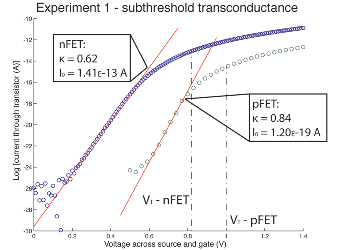
\includegraphics[natwidth=675,natheight=500]{pics/nme_lab2exp1.pdf}
\caption{Reasonable-looking results from lab 2 - measuring $\kappa$ and threshold voltage as described in class (slope of red lines is $\kappa/U_T$) \label{lab2exp1}}
\end{figure}
%-----------------------------------------------
\subsection{On conductance, Early voltage, and mismatch}
Not all transistors behave exactly the same. In fact, it's not easy to find two that do. We call this \emph{device mismatch}. It's primarily a function of the randomness involved in the doping procedure, which is a diffusion process. Because of this, we cannot ensure that any two transistors have the same response characteristics without testing them and finding two that are close enough. We simply cannot control the process that well. There is also uncertainty with dimension tolerances\footnote{In any manufacturing process, a dimension will be produced to a tolerance of $\pm\varepsilon$, so this inherent variation in physical dimensions is going to change the behavior of the transistor ($I_0$ is a function of width and length, remember?)}.\\ \\
This becomes a problem if you design a circuit that is very sensitive to device response characteristics and relies on symmetry between certain devices within the circuit. There are ways to mediate or minimize the problem, but  basically it manifests itself as deviation from an ideal behavior (lateral translation of output vs input plots, threshold variation, etc).\\ \\
Another non-ideal behavior of transistors produces what we call the \emph{Early voltage}\footnote{Named after a person, not a temporal relation}. We said earlier that a transistor does not increase its output current for higher \emph{drain-source} voltages after passing the saturation voltage. This is not actually true, especially for short length MOSFETs. In the above threshold saturation regime, increasing drain voltage beyond the saturation point extends the pinchoff region\footnote{See p. 67, ``Saturation Region'' section for a description of the \emph{pinchoff region}. Really, all you need to remember about the Early voltage is 1) what it does to your output, 2) how to calculate it, and 3) that it's more pronounced in short transistors} further into the channel away from the drain, decreasing the effective length of the transistor and thus increasing its output current. To calculate it, you simply measure the current through a transistor while sweeping the drain voltage. Extrapolate a line from where the saturation region has flattened out and see where it hits the x-axis. This will be the negative Early voltage\footnote{See p.76, Fig 3.16}. The slope of this line is also the \emph{drain conductance} of the transistor at this point, represented as
\begin{equation}
g_{ds} = \frac{\partial I_{ds}}{\partial V_{ds}} = \frac{I}{V_e}
\label{gDrainEqn}
\end{equation}
\\
As transistor length increases, so does Early voltage. The ideal transistor would have an Early voltage of $V_e = \infty$ (horizontal slope, no x-intercept). More imperfections are discussed in the textbook section 3.5 (p. 75), but these are the most important two. It's good to be aware of the other effects (and you have to discuss them in one or two of the lab writeups), but they make fewer appearances throughout the course. The important thing is to understand how mismatch can affect your circuit and what kind of change in behavior you would expect to see for mismatch showing up in any given transistor.\\ \\
While \emph{conductance} is on our minds, let's spend another minute on it. We do know what it is in a general sense - it's $R^{-1}$, right? The inverse of the resistance? If $V = IR$, then $R = V/I$ and $g = I/V$. This is all just a very general statement from our old friend Ohm's Law with no transistor-specific properties. These relationships are a little more involved in transistors than in normal, linear resistors, so we take a more dynamic view and call the conductance the partial derivative of the drain current in terms of the voltage of whichever terminal we're interested in. We tend not to move the source around too much, so mostly we talk about the drain conductance, as shown in ~\eqref{gDrainEqn}, and the gate conductance, most often called the \emph{transconductance}. We call it the transconductance because the current we are concerned with does not go through the terminal whose voltage we are changing\footnote{Remember, it's the gate, and no current goes in or out of the gate}.
\begin{equation}
g_{m} = \frac{\partial I}{\partial V_{g}}
\label{gTransEqn}
\end{equation}
To get conductance expressions, you simply differentiate your relevant current equation, like ~\eqref{subSatEqn}, in terms of the relevant voltage.\\ \\
That pretty well covers the basics of subthreshold behavior, though probably not everything. I didn't plan this thing out all that well. There's also some stuff about $\kappa$ not actually being constant, but you'll see that in the labs.
%-----------------------------------------------
%-----------------------------------------------
\section{Above threshold behavior}
Above threshold we have a different phenomenon. We established that subthreshold current moves around because of diffusion - moving across concentration gradients. Once we get above threshold, the transistor goes into \emph{strong inversion} and the electric field from drain to source takes over and \emph{drift} is the primary motive force. Once you get the basics of chapters 2 and 3, the rest of the course is extrapolating and applying it. So really focus on learning the material in these two chapters - you will be expected to know it well and be able to use that knowledge on the fly during lab sessions.

\subsection{On current equations, $\kappa$, and conductances}
First off, $\kappa$. Once the transistor goes into strong inversion\footnote{This is where the gate voltage is high enough to attract minority carriers so their concentration in the channel is higher than the dopant concentration}, surface potential $\psi_s$ is pretty well coupled with gate potential, so we set $\kappa$ to 1\footnote{A little more technically: any change in $\psi_s$ is due to a change in inversion charge (mobile electron concentration), not depletion charge (fixed ions), and $\kappa$ is limited to describing static charges, being based on capacitances and all}. We will no longer have $\kappa$ in our equations, but another little guy - $\beta$ - gets introduced as a modified version of $I_0$. We are now above threshold, but we still have the ohmic/linear/triode regime and the saturation regime.\\ \\
So current is now tumbling down the electric field between the source and drain, being pushed along by our old friend the electric field. This means the current will flow according to the rules that govern charges moving in a field, with the slight caveat that it happens inside matter, not in the ubiquitous vacuum we studied in undergrad. So what are the main points of these rules? Well, we have $I_{ds}$ as a product of carrier mobility, charge density, and electric field. When we expand the terms we get
\begin{equation}
I_{ds} = \mu C_{ox}\frac{W}{L}(V_{gs} - V_T)V_{ds} = \beta(V_{gs} - V_T)V_{ds}
\label{abvTriodeEqn}
\end{equation}
where $V_T$ is the threshold voltage and $\mu$ is electron mobility (previously hidden inside $I_0$). And look at that! $I_{ds}$ has a linear dependence on both $V_{gs}$ and $V_{ds}$. No wonder they call it the \emph{linear} regime. So as long as you hold one of those two voltages constant and sweep the other, you can easily measure $\beta$ as the slope of the line divided by the voltage that is being held constant (either drain or gate). If you recall, when a transistor is subthreshold, it goes from triode to saturation regime at the same drain voltage ($4U_T$), regardless of gate voltage. Above threshold we don't get that. That saturation $V_{ds}$ now depends on $V_{gs}$ - for higher $V_{gs}$ you get a higher saturation voltage $V_{dsat}$\footnote{$V_{dsat} = V_{gs} - V_T$}.\\ \\
Say we put $V_{ds}$ higher than $V_{dsat}$, so we're in the saturation regime of above threshold. The current equation changes to
\begin{equation}
I_{ds} = \frac{\beta}{2}(V_{gs} - V_T)^2
\label{abvSatEqn}
\end{equation}
with the same $\beta$ as before. Remember this, you will likely get asked this at some point: \textsl{subthreshold current is an exponential function of voltage, but above threshold it's linear in the linear region and \emph{quadratic} in the saturation regime}. Also, try to remember \emph{which} voltages it's linear or quadratic or exponential with. Here if we plot the square root of the current against $V_{gs}$, the slope of the line is a nice, friendly $\sqrt{\beta/2}$. All of this is shown pretty clearly in the slides.\\ \\
So, $\kappa$ has not completely disappeared. I know, I know, we said it's no longer relevant to the surface potential. That is true. Now, however, it has a hand in controlling the threshold voltage, along with $V_s$ as $V_T = V_{T0} + \frac{V_s}{\kappa}$. The class does not really spend much time on that, though.\\ \\
%--------------------------------------------
\subsection{Another word on current dependencies}
The full above threshold equation, which contains all the information we need to derive both ~\eqref{abvTriodeEqn} and ~\eqref{abvSatEqn} is
\begin{equation}
I = \frac{\beta}{2}\big[((V_g - V_{T0}) - V_s)^2 - ((V_g - V_{T0}) - V_d)^2\big] \label{abvThreshEqn}
\end{equation}
which we can look at as the difference between forward (the half with $V_s$) and reverse (the half with $V_d$) currents. We have to do some algebra to get this in the form of ~\eqref{abvTriodeEqn}, but essentially the current is product of inversion charge in the channel (which is linear in $V_g - V_{T0}$) and the electric field across the channel (which is linear in $V_{ds}$).\\ \\
In saturation, $V_d$ is high enough that any electron that gets near the drain is instantly sucked up into it, so that end of the channel actual goes subthreshold\footnote{This is the \textsl{pinchoff} region} because the concentration of mobile carriers is so low (they all get pulled into the drain by the electric field arising from the voltage between the channel and the drain, where they are whisked away to $V_{dd}$ and the greener pastures that await them there).\\ \\
Overall, current is a proportional to inversion charge concentration  and the electric field\footnote{$I = J_{drift}Width_{channel}Depth_{channel} = \mu W Q_i \mathcal{E} \propto Q_i \frac{d}{dz}Q_i = \frac{d}{dz}Q_i^2$}. Integrating this relationship over the length of the channel gives $I \propto Q_i^2 = (Q_s^2 - Q_d^2)$\footnote{Inversion charge concentrations at source and drain ends of channel}. Saturation says $Q_d \to 0$ \footnote{Remember? all electrons that make it to that end immediately bugger off through the drain}, so current is only a function of $Q_s$ and we drop off the second half of ~\eqref{abvThreshEqn} to get ~\eqref{abvSatEqn}. \\ \\
I found it very helpful to sit down with the equations and trace dependencies back to their roots\footnote{Letting you do this is where the book really earns its keep}. For example, you look at ~\eqref{abvThreshEqn} to see how current depends on voltages. You then look in the book and find that the voltages are functions of inversion charge. You look farther back to see what inversion charges are functions of, and so on. Without knowing what phenomena give rise to a given term, it's hard to build an intuition for any of this. But maybe that's just me.\\ \\
I'll only mention conductances here to say that we calculate them the same way as before - differentiate your current in terms of whatever your relevant voltage is. And there you have it. Study your labs.
%-----------------------------------------------
%-----------------------------------------------




\section{Logarithmic I/V converter}
%David
We can call this a circuit, but this is simply what a transistor does in subthreshold - converts the log of the current to a voltage\footnote{Or vice versa - that's a current source}. We can think of the transistor as having three variable parameters: $V_g$, $V_s$, and $I_{ds}$\footnote{We ignore $V_d$ for now}. The circuit is just a single transistor where current into the drain is our input and the output is either the gate or source voltage. The equations are simply algebraic manipulations of the subthreshold saturation equation ~\eqref{subSatEqn}.
\begin{equation}
V_s = \kappa V_g - U_T \log \left(\frac{I}{I_0}\right)
\end{equation}
\begin{equation}
V_g = \frac{1}{\kappa}\left( V_s + U_T \log \left(\frac{I}{I_0}\right) \right)
\end{equation}
In each case, you fix the voltage that is not being measured at a constant value. \emph{Important note:} due to the infinite impedance between gate and channel, $V_g$ (determined  - by definition - by charge on the gate) cannot be directly influenced by the input current. For this version to work, there must be feedback between the gate and the drain, which can be accomplished by shorting the two together (see Figure~\ref{diodeConn}). This is a \emph{diode-connected} transistor, called such because it functionally has only two terminals, like a diode.\\ \\
Doing this has two effects. First, it ensures that the transistor stays in the saturation regime by maintaining a reverse bias betweeen drain and channel. Second, if we force a certain current through, this will set the drain voltage and then necessarily the gate voltage (because the two are shorted together). See? Positive feedback from drain to gate (and therefore negative feedback from gate to drain).
%-----------------------------------------------



\section{Current source}
%David
This is another iteration of ``we call this a circuit but really it is simply what transistors do.'' In this case, $V_s$, $V_d$, and $V_g$ are set to constant values and $I_{ds}$ is our output. In practice, we tie $V_s$ to ground, put $V_g$ at some value less than 0.7V (to keep it subthreshold), and $V_d$ is put above 100mv to keep it in saturation. If we use a long transistor we can ignore Early voltage effects.\\ \\
Technically this is a current \emph{sink}, not a current \emph{source} because the current is pulled into the drain from above\footnote{``Above'' refers to ``closer to $V_{dd}$''}. To have a current source that will go higher in the circuit than whatever is consuming your current, you simply use a pFET instead of an nFET, tie the source to $V_{dd}$, and set gate voltage such that $V_g > V_{dd} - 0.7$. In either case the equation to calculate output current is by definition the subthreshold saturation current $I_{ds} = I_0 \exp ( (\kappa V_g - V_s)/U_T )$.
%------Diode-connected transistor-------
\begin{figure}[ht]
 \centering
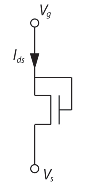
\includegraphics[natwidth=185,natheight=375]{pics/nme_diodeConn_transistor.pdf}
\caption{Diode-connected nFET \label{diodeConn}}
\end{figure}



\section{Current Mirror}
% Joachim
The current mirror circuit is built by connection the gate of a diode-connected transistor to the gate of another transistor.
Both transistors have a fixed source voltage, are in saturation, and act as a current source.


\begin{figure}[htbp]
  \centering
  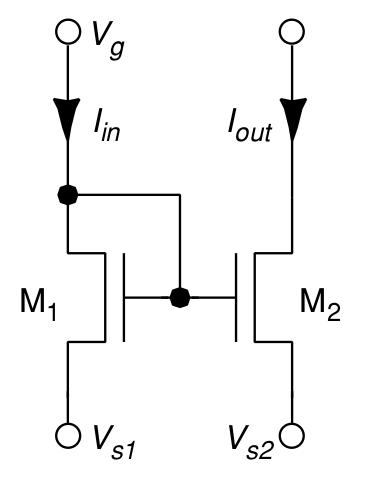
\includegraphics[scale=1]{pics/current_mirror_vlsi.png}
  \caption{nFET Current Mirror \cite{book:VLSI}}
  \label{fig:nFET_Current_Mirror}
\end{figure}\bigskip

\begin{itemize}
\item M1: Diode connected transistor
\item Input current $I_{in}$ sets common gate voltage $V_g$, hence also sets $I_{out}$
\end{itemize}

\subsection{Scaling of $I_{in}$ vs $I_{out}$}
\begin{itemize}
\item By choosing different source potentials $V_{s1}$ and $V_{s1}$
\subitem Leads to exponential scaling: $I_{out}=e^{V_{s1}-V_{s2}/U_T} \cdot I_{in}$
\item By choosing different transistor sizes
\subitem The current scales linearly with transistor size difference 
\subitem Important: Fixed transistor width vs. length ratio
\end{itemize}

\subsection{Above Threshold Operation}
Input vs. output currents depends mainly on drain voltage of $M_1$ and $M_2$, because of larger Early effect. The dependence on the source voltage is much weaker.\\
With bidirectional input, the current mirror can be used as half wave rectifier, because the input transistor has high impedance in the opposite direction.

\begin{figure}[htbp]
  \centering
  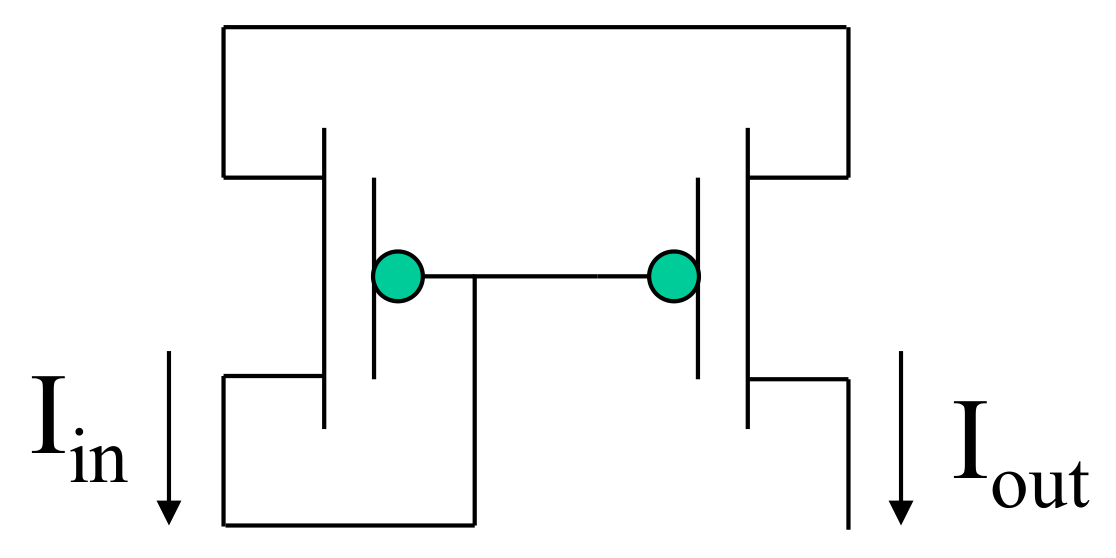
\includegraphics[scale=0.5]{pics/current_mirror_pfet.png}
  \caption{pFET Current Mirror \cite{lec4}}
  \label{fig:pFET_Current_Mirror}
\end{figure}\bigskip





\section{Source Follower}
%Joachim
The source follower
\begin{itemize}
\item Transforms a weakly-driven voltage signal into a more strongly-driven voltage signal
\item Is a two transistor circuit consisting of two MOSFET in series
\item Consists of a fixed current source that is connected to the source of another MOSFET in saturation 
\item Linearly transforms a voltage $V_{in}$ at a high impedance input terminal $M_1$ into a voltage at a lower impedance output terminal $V_{out}$
\subitem M1 source is equal to $V_{out}$
\subitem $V_{out}$ is able to drive larger loads
\end{itemize}

\begin{figure}[htbp]
  \centering
  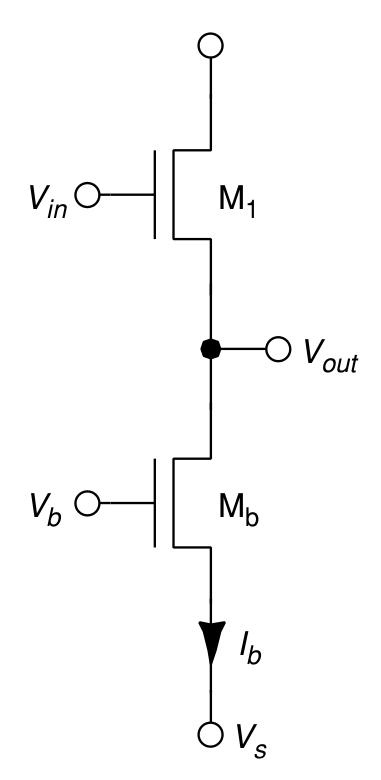
\includegraphics[scale=1]{pics/source-follower.png}
  \caption{Source Follower Circuit \cite{book:VLSI}}
  \label{fig:Source_Follower_Structure}
\end{figure}

\subsection{Proper Operation Requirements}
Saturation of the biasing transistor: $V_{out} > V_s + 4U_T$\\
that is $V_{in} > K_{n}^{-1}(\kappa_b V_b + 4U_T)$

\subsection{Subthreshold Operation}
In subthreshold, the output voltage changes according to:
\begin{equation}
V_{out}=\kappa_n V_{in} - U_T log(\frac{I_b}{I_{n0}}) = \kappa_n V_{in} - \kappa_b V_b + V_s
\end{equation}
\begin{center}
$\kappa_b$ is the subthreshold slope factor of $M_b$\\
\end{center}
$V_{out}$ is linearly related to $V_{in}$
\begin{itemize}[label={}]
\item $1 >\kappa_n >0$
\item $V_{out}$ has a fixed offset that depends on bias current $I_b$
\end{itemize}

\subsection{Gain}
$V_{out}$ follows $V_{in}$ with gain of $K_n$\\
Important: $K_n$ is not constant due to the body effect of $M_n$

%Joachim End








\section{Differential Pair}
%Doris

The Differential Pair circuit, as shown in Figure \ref{fig:Differential_pair_circuit}, is composed of two source followers with a common Fixed Current Source, $M_b$, with the bias voltage, $V_b$. The transistors, $M_1$ and $M_2$, have variable voltage inputs, $V_1$ and $V_2$, respectively, and share a common source, node V, which also acts as the drain of $M_b$. 

\begin{figure}[htbp]
  \centering
  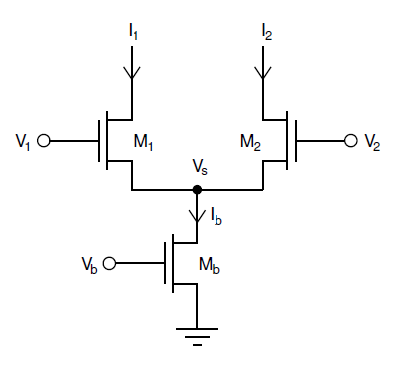
\includegraphics[scale=0.8]{pics/Differential_pair_circuit.png}
  \caption{Differential Pair Circuit}
  \label{fig:Differential_pair_circuit}
\end{figure}


The output current is proportional to the difference in the input voltages according to: 

\begin{equation}
I_1 = I_b\frac{e^{\kappa V_1}}{e^{ \kappa V_1}+e^{\kappa V_2}} = \frac{I_b}{1+ e^{\kappa(V_2-V_1)}}  \geq 0
\end{equation}
\begin{equation}
I_2 = \frac{I_b}{1+e^{\kappa(V_1-V_2)}} \geq 0
\end{equation}

Before the currents $I_1$ and $I_2$ are input, the Differential pair is off because the drain of $M_b$ (node V) is off. Once $I_1$ and $I_2$ are on and in saturation, they will charge node V to turn on $M_b$ and put $I_b$ into saturation. The transistor with the lower input voltage ($V_1$ or $V_2$) will act as a drain choke and allow less current through its drain. The losing transistor will see its source voltage (node V) increase and thus fall out of saturation. 


 \begin{figure}[htbp]
  \centering
  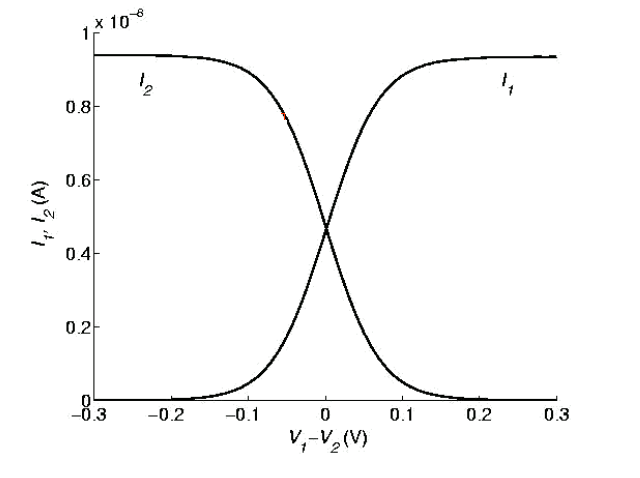
\includegraphics[scale=0.6]{pics/I-V_characteristics_of_Differential_pair.png}
  \caption{I-V characteristics of Differential pair}
  \label{fig:I-V_characteristics_of_Differential_pair}
\end{figure}




\begin{figure}[htbp]
  \centering
  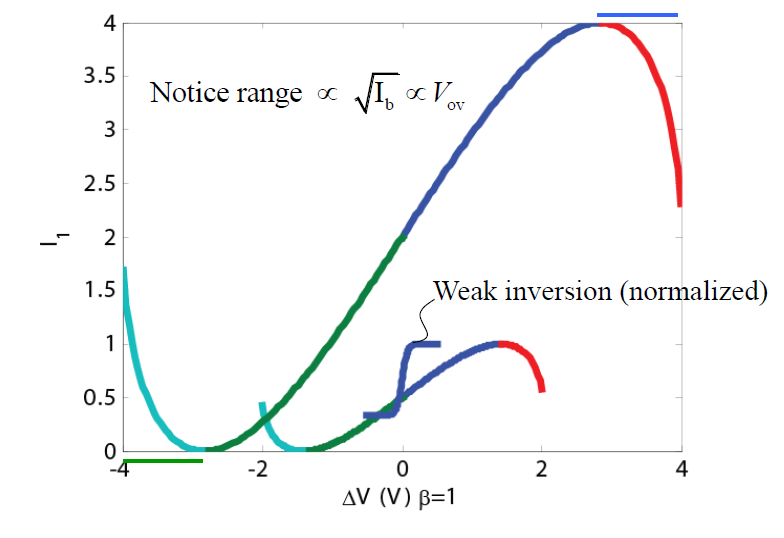
\includegraphics[scale=0.6]{pics/Differential_pair_in_weak_strong_inversion.png}
  \caption{I-V characteristics of Differential pair with reference to input voltage difference in weak $\&$ strong inversion}
  \label{fig:Differential_pair_in_weak_strong_inversion}
\end{figure}


\begin{figure}[htbp]
  \centering
  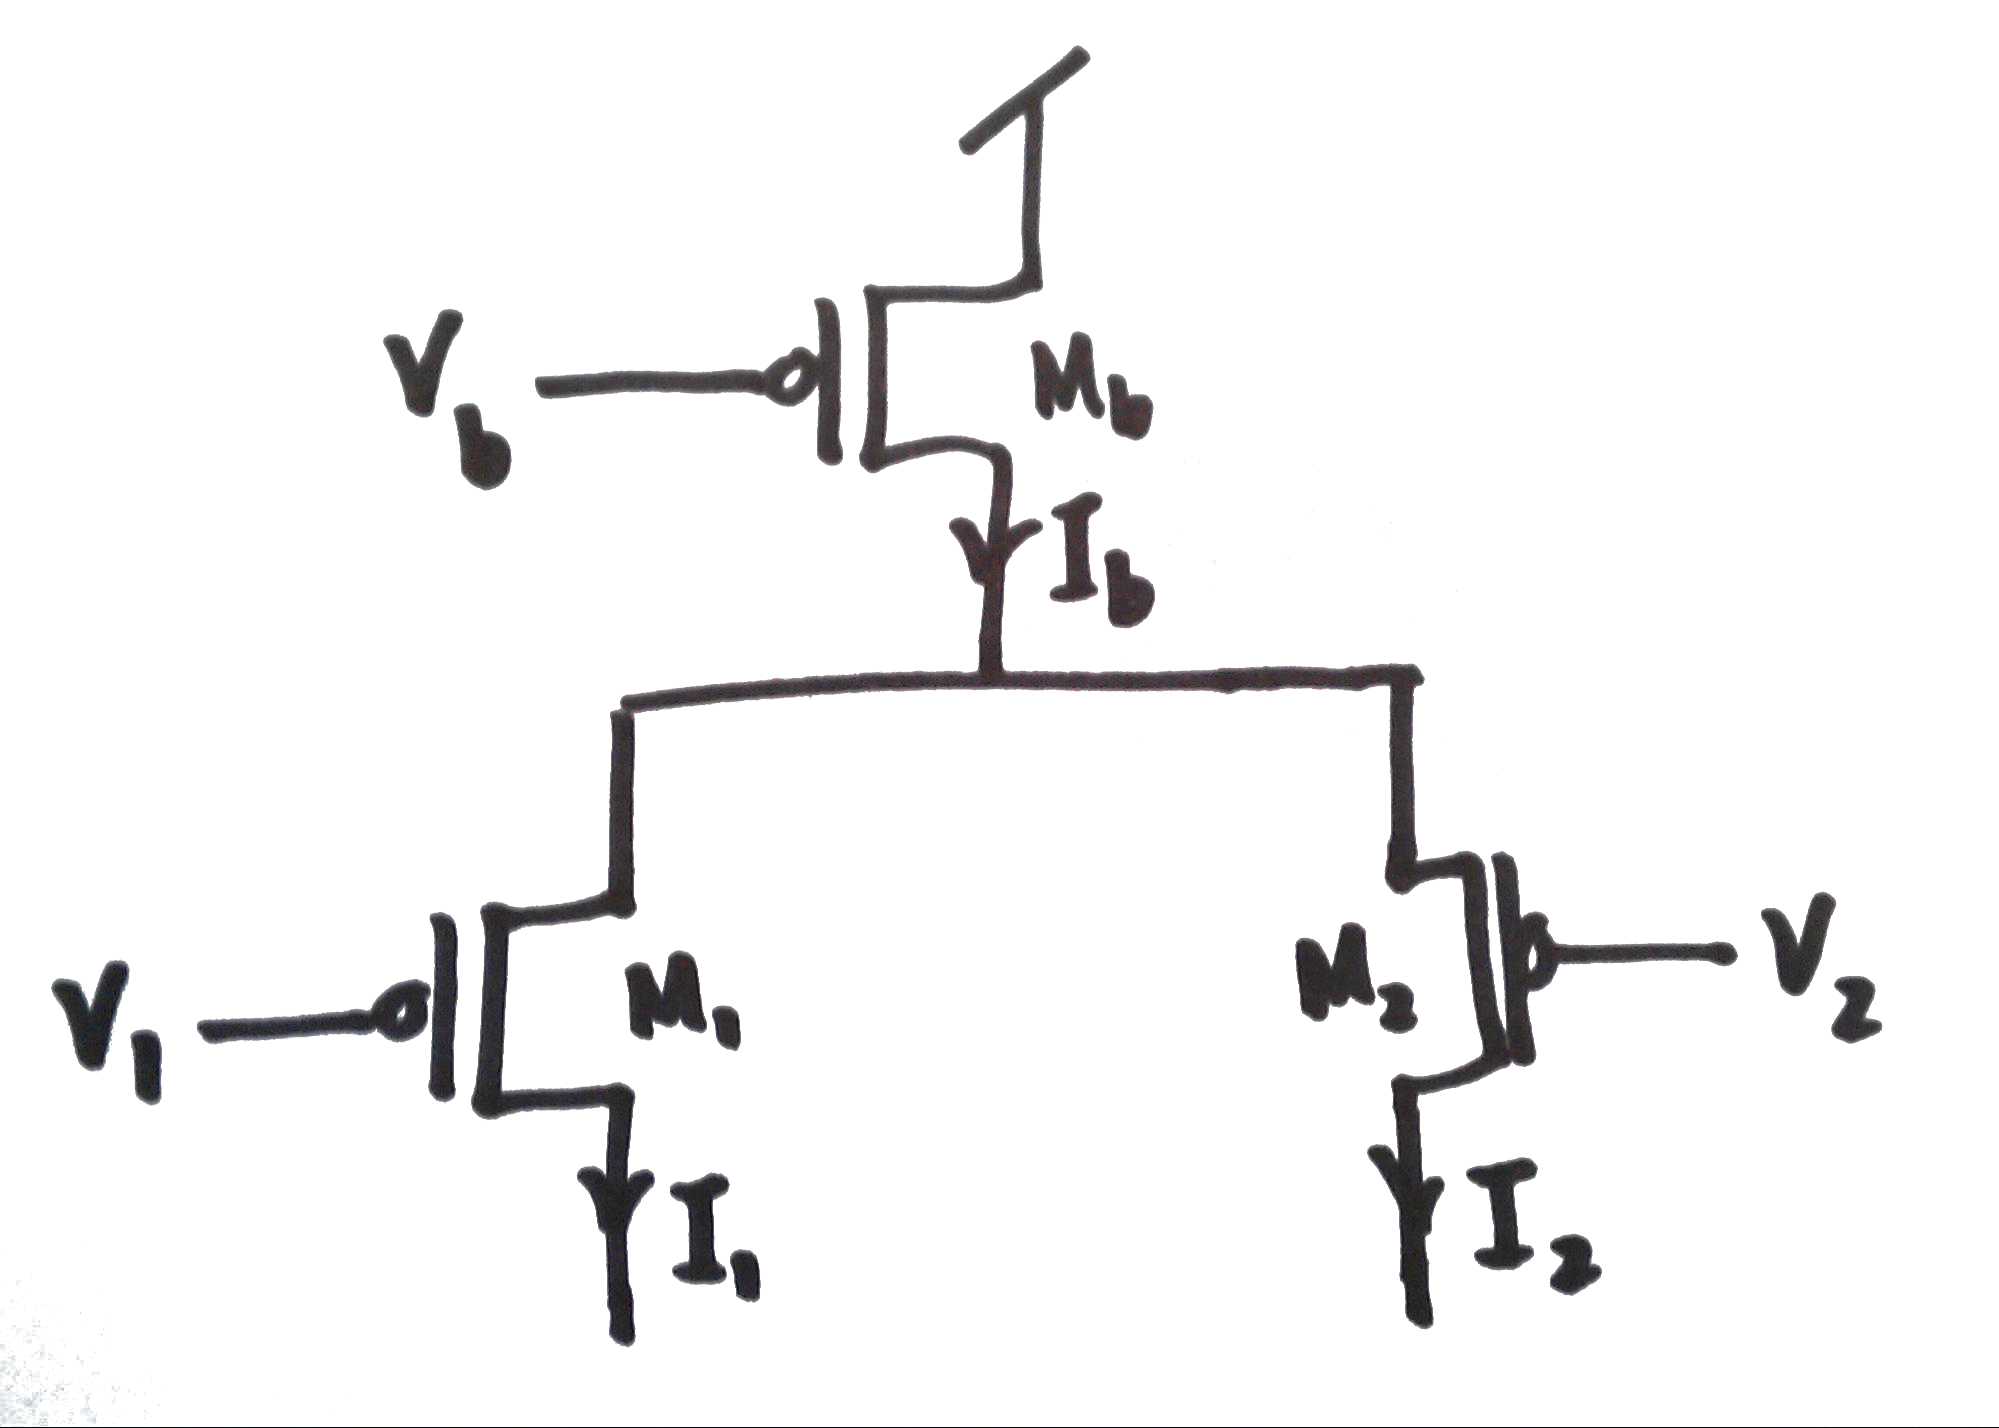
\includegraphics[scale=0.2]{pics/pFET_Differential_pair_circuit.png}
  \caption{pFET Differential pair $\rightarrow$ flipped w bias on top connected to Vdd, and M1, M2 sinking current}
  \label{fig:pFET_Differential_pair_circuit}
\end{figure}



\section{Current Conveyor}
% Doris
The Current Conveyor, also commonly known as a Buffered Current Mirror, consists of two transistors. where the $M_1$ gate is tied to the $M_2$ drain, and the $M_2$ gate is tied to the $M_1$ source as shown in Figure \ref{fig:Current_Conveyor_circuit}.

\begin{figure}[htbp]
  \centering
  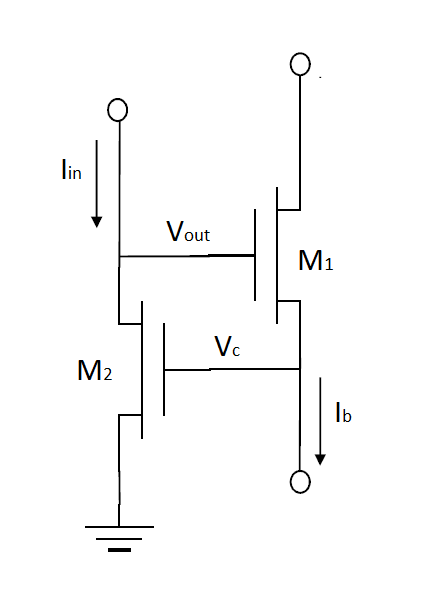
\includegraphics[scale=0.5]{pics/Current_Conveyor_circuit.png}
  \caption{Current Conveyor circuit}
  \label{fig:Current_Conveyor_circuit}
\end{figure}
The Current Conveyor acts like a source follower ($M_1$) whose output terminal is tied to the gate of a current sink ($M_2$). The input current, $I_{in}$, will charge $V_{out}$ to turn on $M_1$ whose current will charge $V_c$, turning on $M_2$ until $M_2$ sinks $I_{in}$. The current being sunk by $M_2$ follows $V_c$ according to:

\begin{equation}
I =  e^{\kappa*V_c} \geq 0
\end{equation}  



\section{Current Correlator}
%Doris

\begin{figure}[htbp]
  \centering
  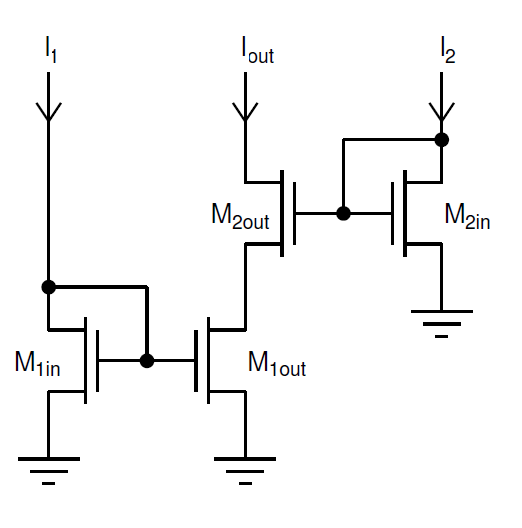
\includegraphics[scale=0.7]{pics/Current_correlator_circuit.png}
  \caption{Current correlator circuit}
  \label{fig:Current_correlator_circuit}
\end{figure}

The Current Correlator is comprised of two stacked current mirrors that have the output of one mirror ($M_2$) lead into the drain of the other mirror ($M_1$). Currents, $I_1$ and $I_2$, are sunk through the diode connected half of both mirrors, pulling $V_1$ and $V_2$, respectively, so that they follow: 

\begin{equation}
I_{out} = I_o e^{\kappa V_1}\cdot(1-e^{V}) \geq 0
\end{equation}


If $V_1 > V_2$, $M_1$ will sink $I_1$ and pull up the common node voltage V (of the $M_1$ drain voltage and $M_2$ source voltage), reducing the current through $M_2$. Thus $I_{out}$ settles at a self normalized product between $I_1$ and $I_2$. 

\begin{equation}
I_{out} = \frac{I_1 \cdot I_2}{I_1+I_2} \geq 0
\end{equation}

However, if $V_1$ is off, $I_2$ will charge common node V until $M_2$ shuts off once $V>V_{d_M2}+4U_t$. Likewise, if $M_2$ is off, the drain of $M_1$ will be off. 

\begin{figure}[htbp]
  \centering
  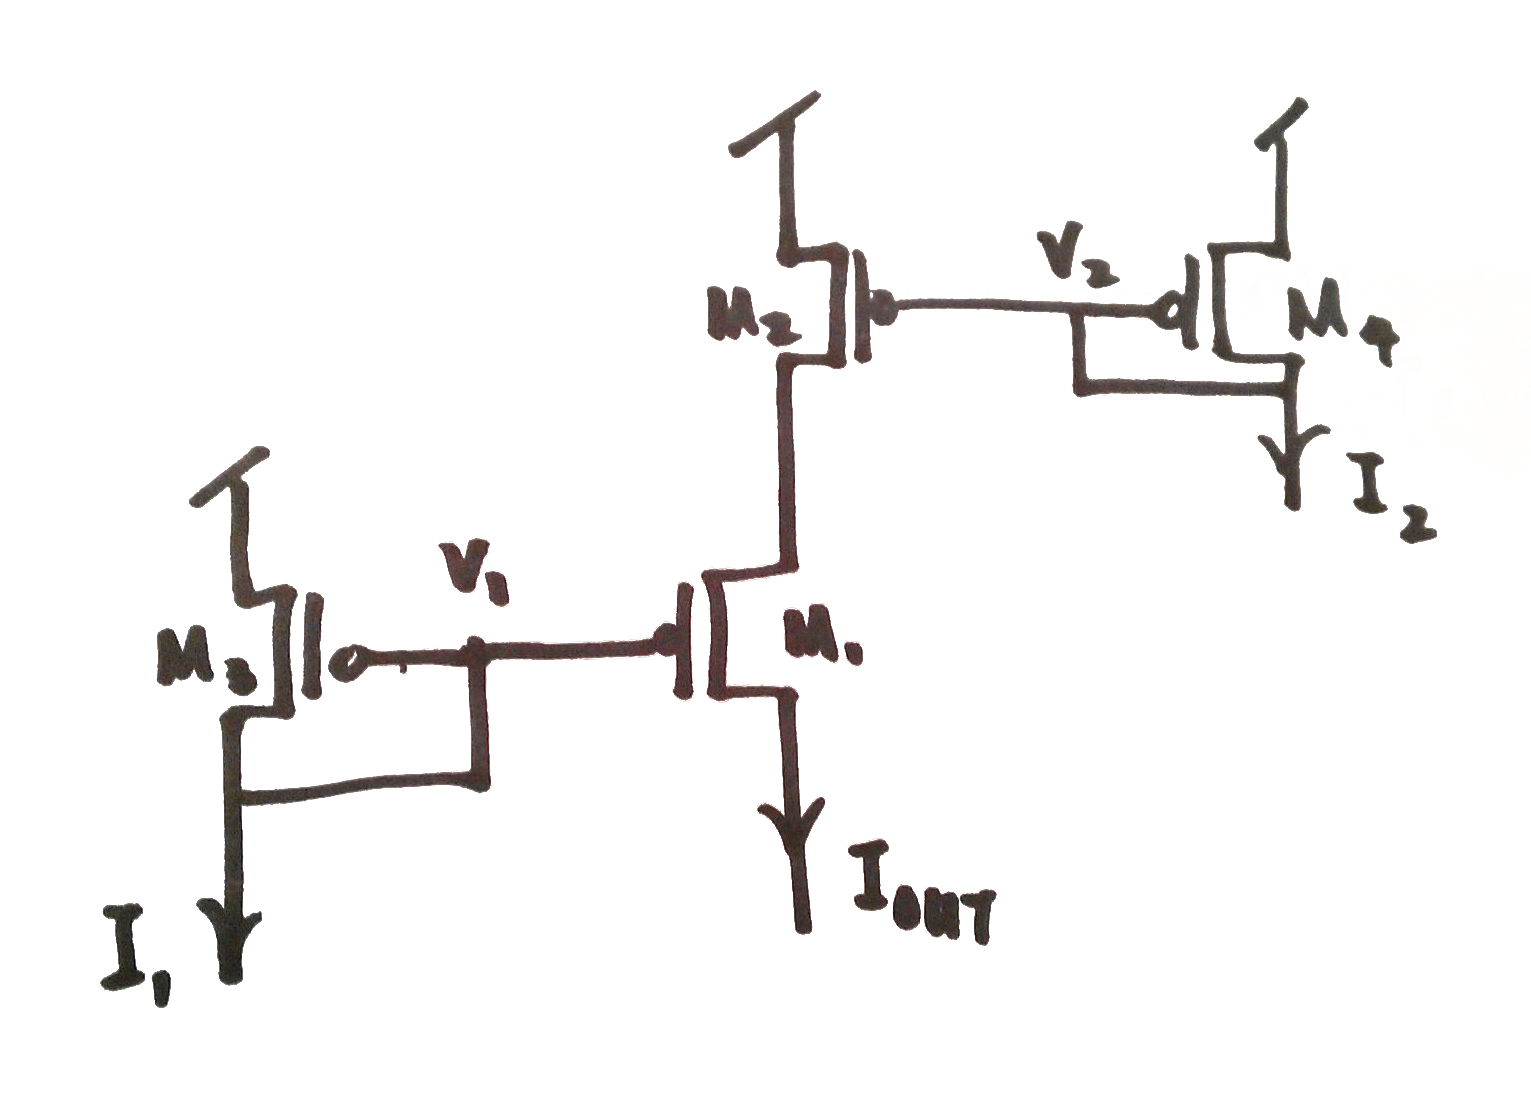
\includegraphics[scale=0.2]{pics/pFET_Current_correlator_circuit.png}
  \caption{pFET Current correlator$ \rightarrow$ two stacked pFET mirrors with 3 current sinks}
  \label{fig:pFET_Current_correlator_circuit}
\end{figure}




\section{Bump Circuit}
% Doris

The Bump-Antibump circuit is comprised of a Differential Pair with the gates of the input transistors tied to the gates of two stacked transistors. 

\begin{figure}[htbp]
  \centering
  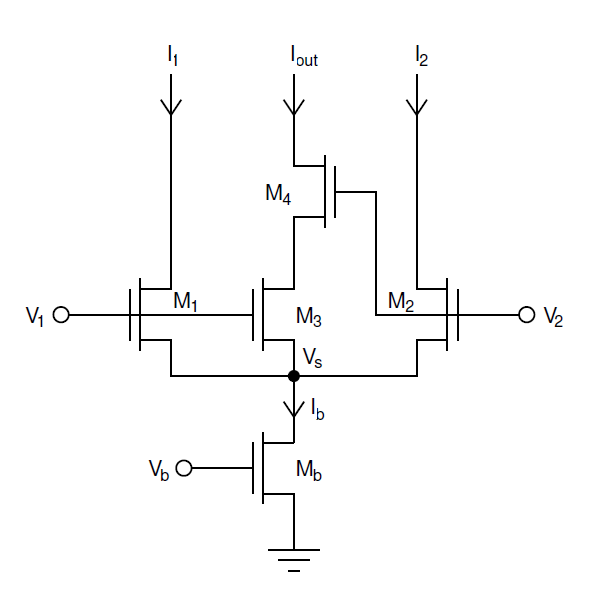
\includegraphics[scale=0.7]{pics/Bump-Antibump_circuit.png}
  \caption{Bump circuit}
  \label{fig:Bump-Antibump_circuit}
\end{figure}

If $V_1 >> V_2$ or $V_2 >> V_1$, then the circuit behaves as a Differential Pair with $I_{out}$ as a function of $V_2 -V_1$.

\begin{equation}
I_{out} = \frac{I_b}{1+\frac{4}{S}cosh^2 \frac{\kappa dV}{2U_T}} \geq 0
\end{equation}

where the transistor geometry factor, 

\begin{equation}
S = \frac{(W/L)_{middle}}{(W/L)_{outer}}
\end{equation}

If the difference between $V_1$ and $V_2$ is small, the stacked transistors will have similarly biased gates, and $I_{out}$ will reflect the sum of the two currents according to:

%shouldn't it be I_b-I_{out}???
\begin{equation}
I_1+I_2 = I_b+I_{out}= \frac{I_B}{1+ \frac{S}{4} cosh^{-2} \frac{\kappa dV}{2U_T}} \geq 0
\end{equation}

If the limit of $I_1$ + $I_2$ is taken as $\delta$ V $\rightarrow$ 0, the sum reaches an absolute minimum at 

\begin{equation}
I_1+I_{2_{min}} = \frac{I_b}{1+\frac{S}{4}} \geq 0
\end{equation}


\begin{figure}[htbp]
  \centering
  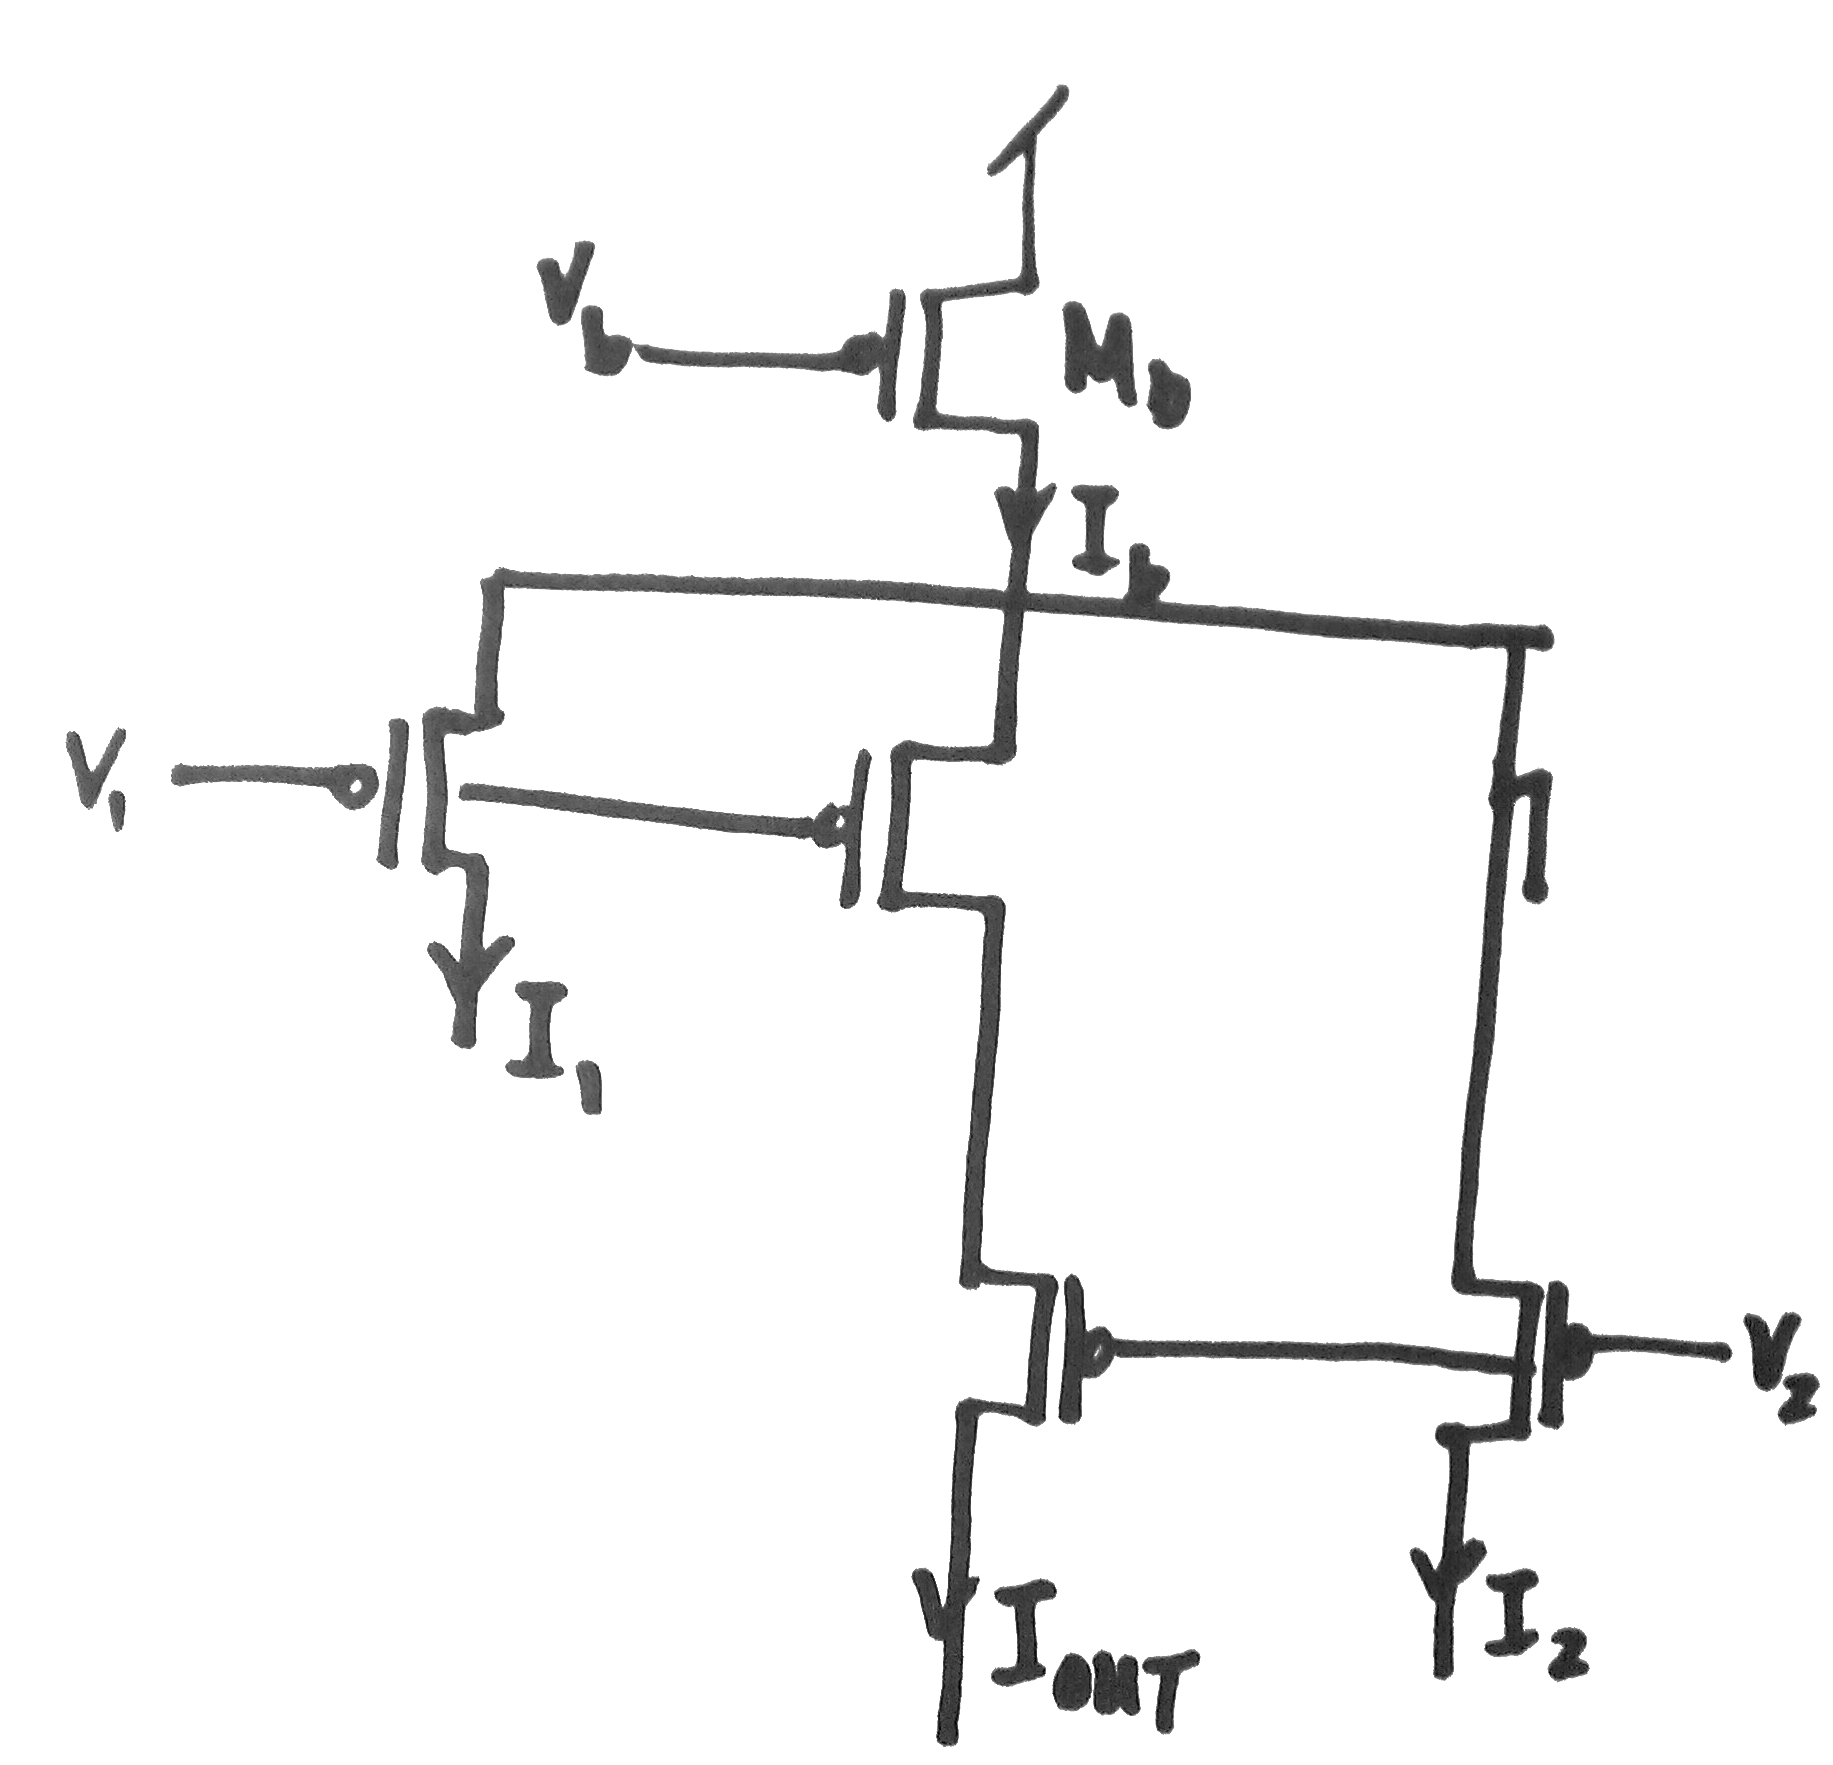
\includegraphics[scale=0.2]{pics/pFET_Bump_circuit}
  \caption{pFET Bump circuit}
  \label{fig:pFET_Bump_circuit}
\end{figure}




\section{Transconductance Amplifier}
%Roland
\begin{figure}[b]
\begin{subfigure} [b]{0.45\textwidth}
  \centering
  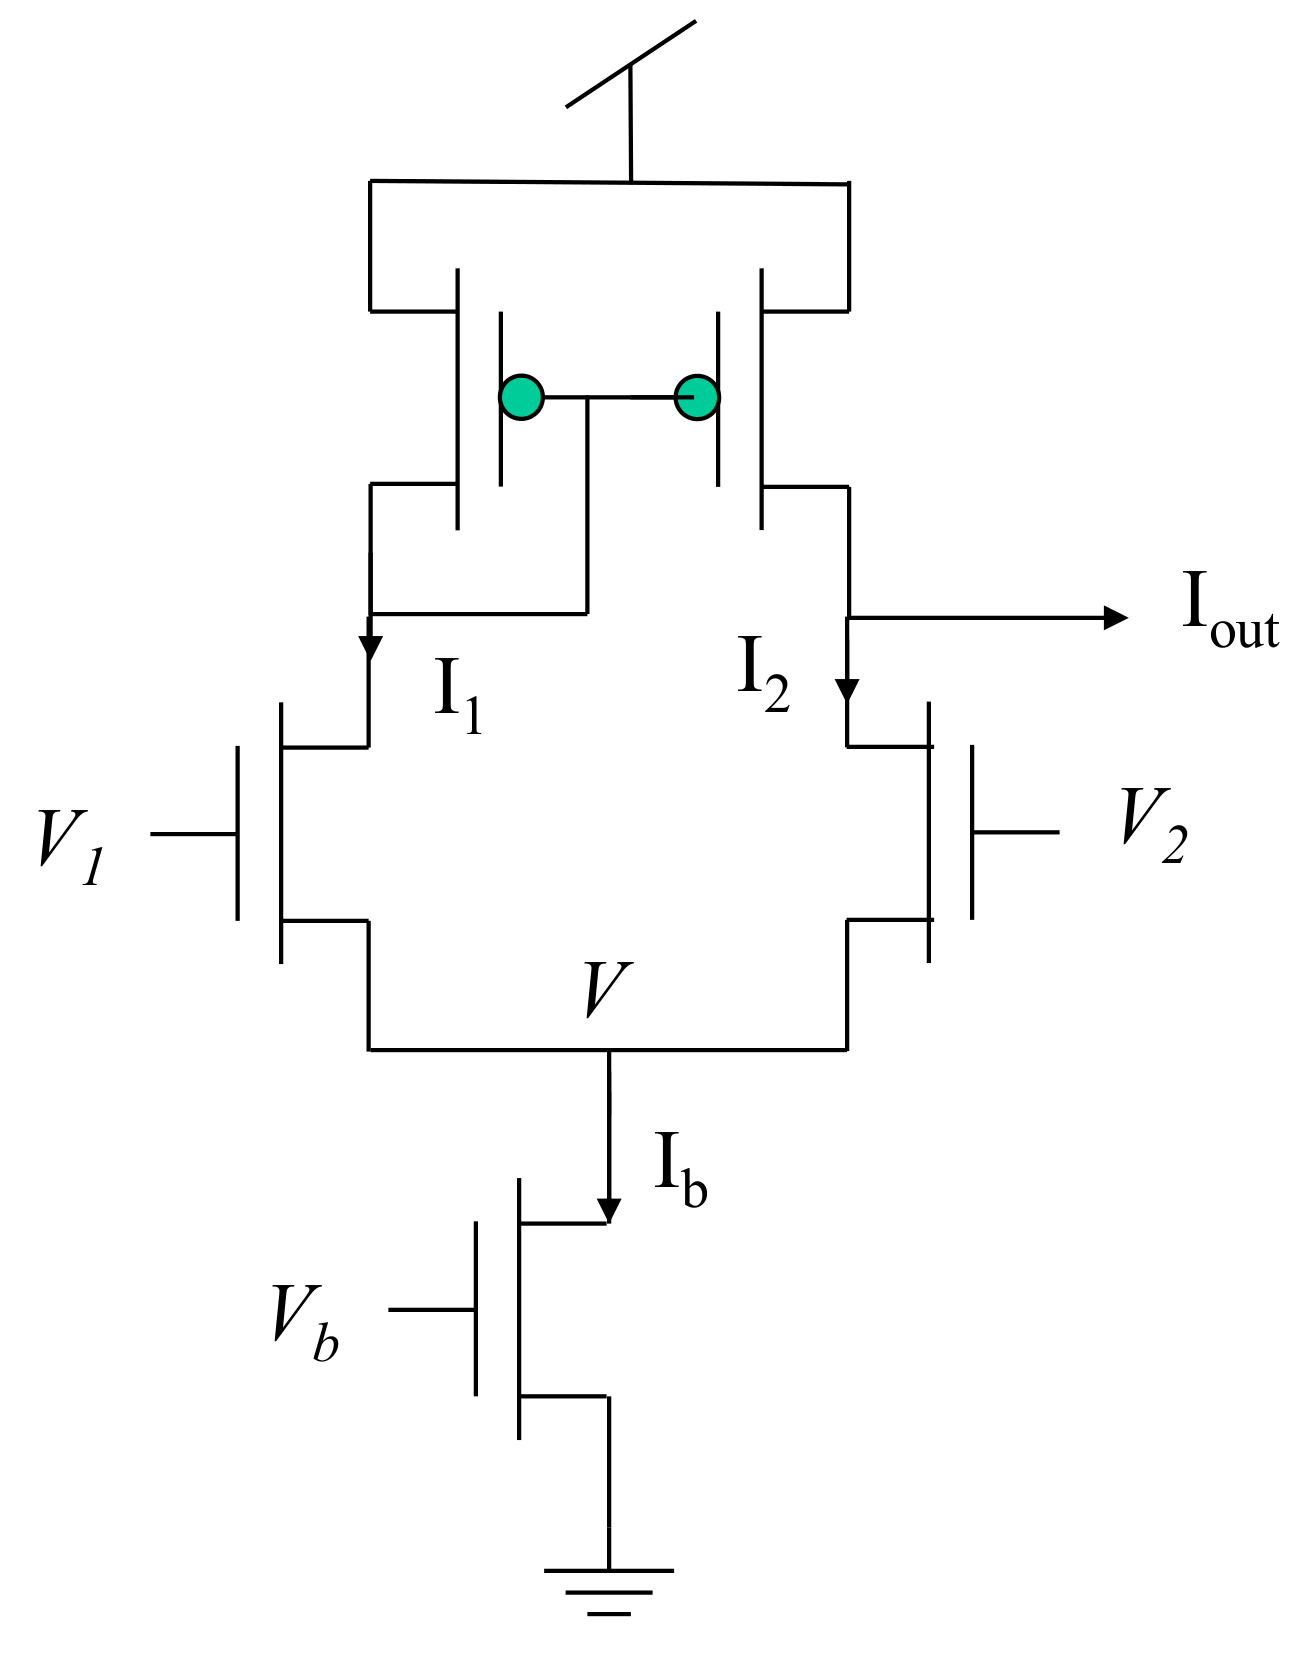
\includegraphics[scale=0.5]{pics/transamp.png}
  \caption{Circuit layout. \cite{lec4}}
  \label{fig:transamp}
\end{subfigure}
	\begin{subfigure} [b]{0.45\textwidth}
	\centering
	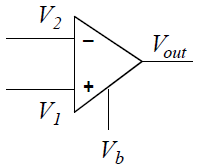
\includegraphics[scale=1]{pics/transcondamp_sym.png}
	\caption{Circuit symbol. \cite{lec5}}
	\label{fig:transamp_sym}
	\end{subfigure}
	\label{fig:transamp_all}
	\caption{A simple transconductance amplifier.}
\end{figure}\bigskip

The simple transconductance amplifier is very easy to understand if you know how the differential pair and the current mirror works, so check back if you don't. 

The bottom part of the transconductance amplifier (Fig. \ref{fig:transamp}) is a differential pair with a current mirror from one of the two outputs to the other one. What now happens is that the current $I_1$ get mirrored on top of $I_2$. We assume that $V_1$ and $V_2$ are not equal, and so aren't $I_1$ and $I_2$. The difference between the two currents then flows in or out of the amplifier in a way that Kirchhoff's current law is fulfilled:
$$I_{out} = I_1 - I_2 = I_b \tanh\left(\kappa \frac{V_1-V_2}{2U_T}\right)$$
Or for a small differential input ($|V_1-V_2| < 200 mV$):
$$ I_{out} \approx g_m \left(V_1-V_2\right) \text{  with  } g_m \approx \frac{\kappa I_b}{2U_T}$$
Since amplifiers are usually used in voltage and not in current mode, we focus on its behavior when the output current $I_{out}$ is fixed. Let's set $V_1 = V_2$ such that $I_{out}$ is zero and keep it there. If we now increase for example $V_2$, the corresponding transistor would drain more current, which can't be provided by the upper transistor since it only mirrors $I_1$. In order to fulfill all transistor equations and Kirchhoff's current law, $V_{out}$ decreases such that the lower transistor is no longer in saturation. Since the transistors behave exponential, even a small change of the input voltages leads to a big change in the output voltage.
\par For this amplifying behavior, it is very important that all transistors operate in saturation region. We already know the common node voltage is 
$ V = \kappa \left(\max \left(V_1, V_2\right)-V_b \right)$ if $|V_1 - V_2| > 4U_T$. Therefore, the saturation condition for the bias transistor is
$\max \left(V_1, V_2\right) > V_b + \frac{4U_T}{\kappa}$. The saturation conditions for the upper and bottom transistors at the output are
$  V_{dd} - V_{out} > 4U_T$ and $V_{out} -V_s > 4U_T$. We see that $V_{out}$ is very restricted (especially towards ground) at the output with
$$\kappa\left(\max \left(V_1, V_2\right)- V_b\right) + 4U_T < V_{out} < V_{dd}-4U_T$$
Outside of this range, the amplifier no longer behaves like an amplifier. The output voltage simply won't change anymore.

Usually, we use amplifiers as depicted in Fig. \ref{fig:transamp_sym}, where 
$$V_{out}=A (V_1 -V_2)$$ 
and we call $A = \frac{g_m}{g_d}$ the amplifiers gain. In subthreshold operation the gain is $A \approx \frac{\kappa V_E}{2U_T}$ and above threshold it is $A \approx \sqrt{\frac{\beta}{I_b}}V_E$.

\section{Wide Range Transconductance Amplifier}

\begin{figure}[htbp]
  \centering
  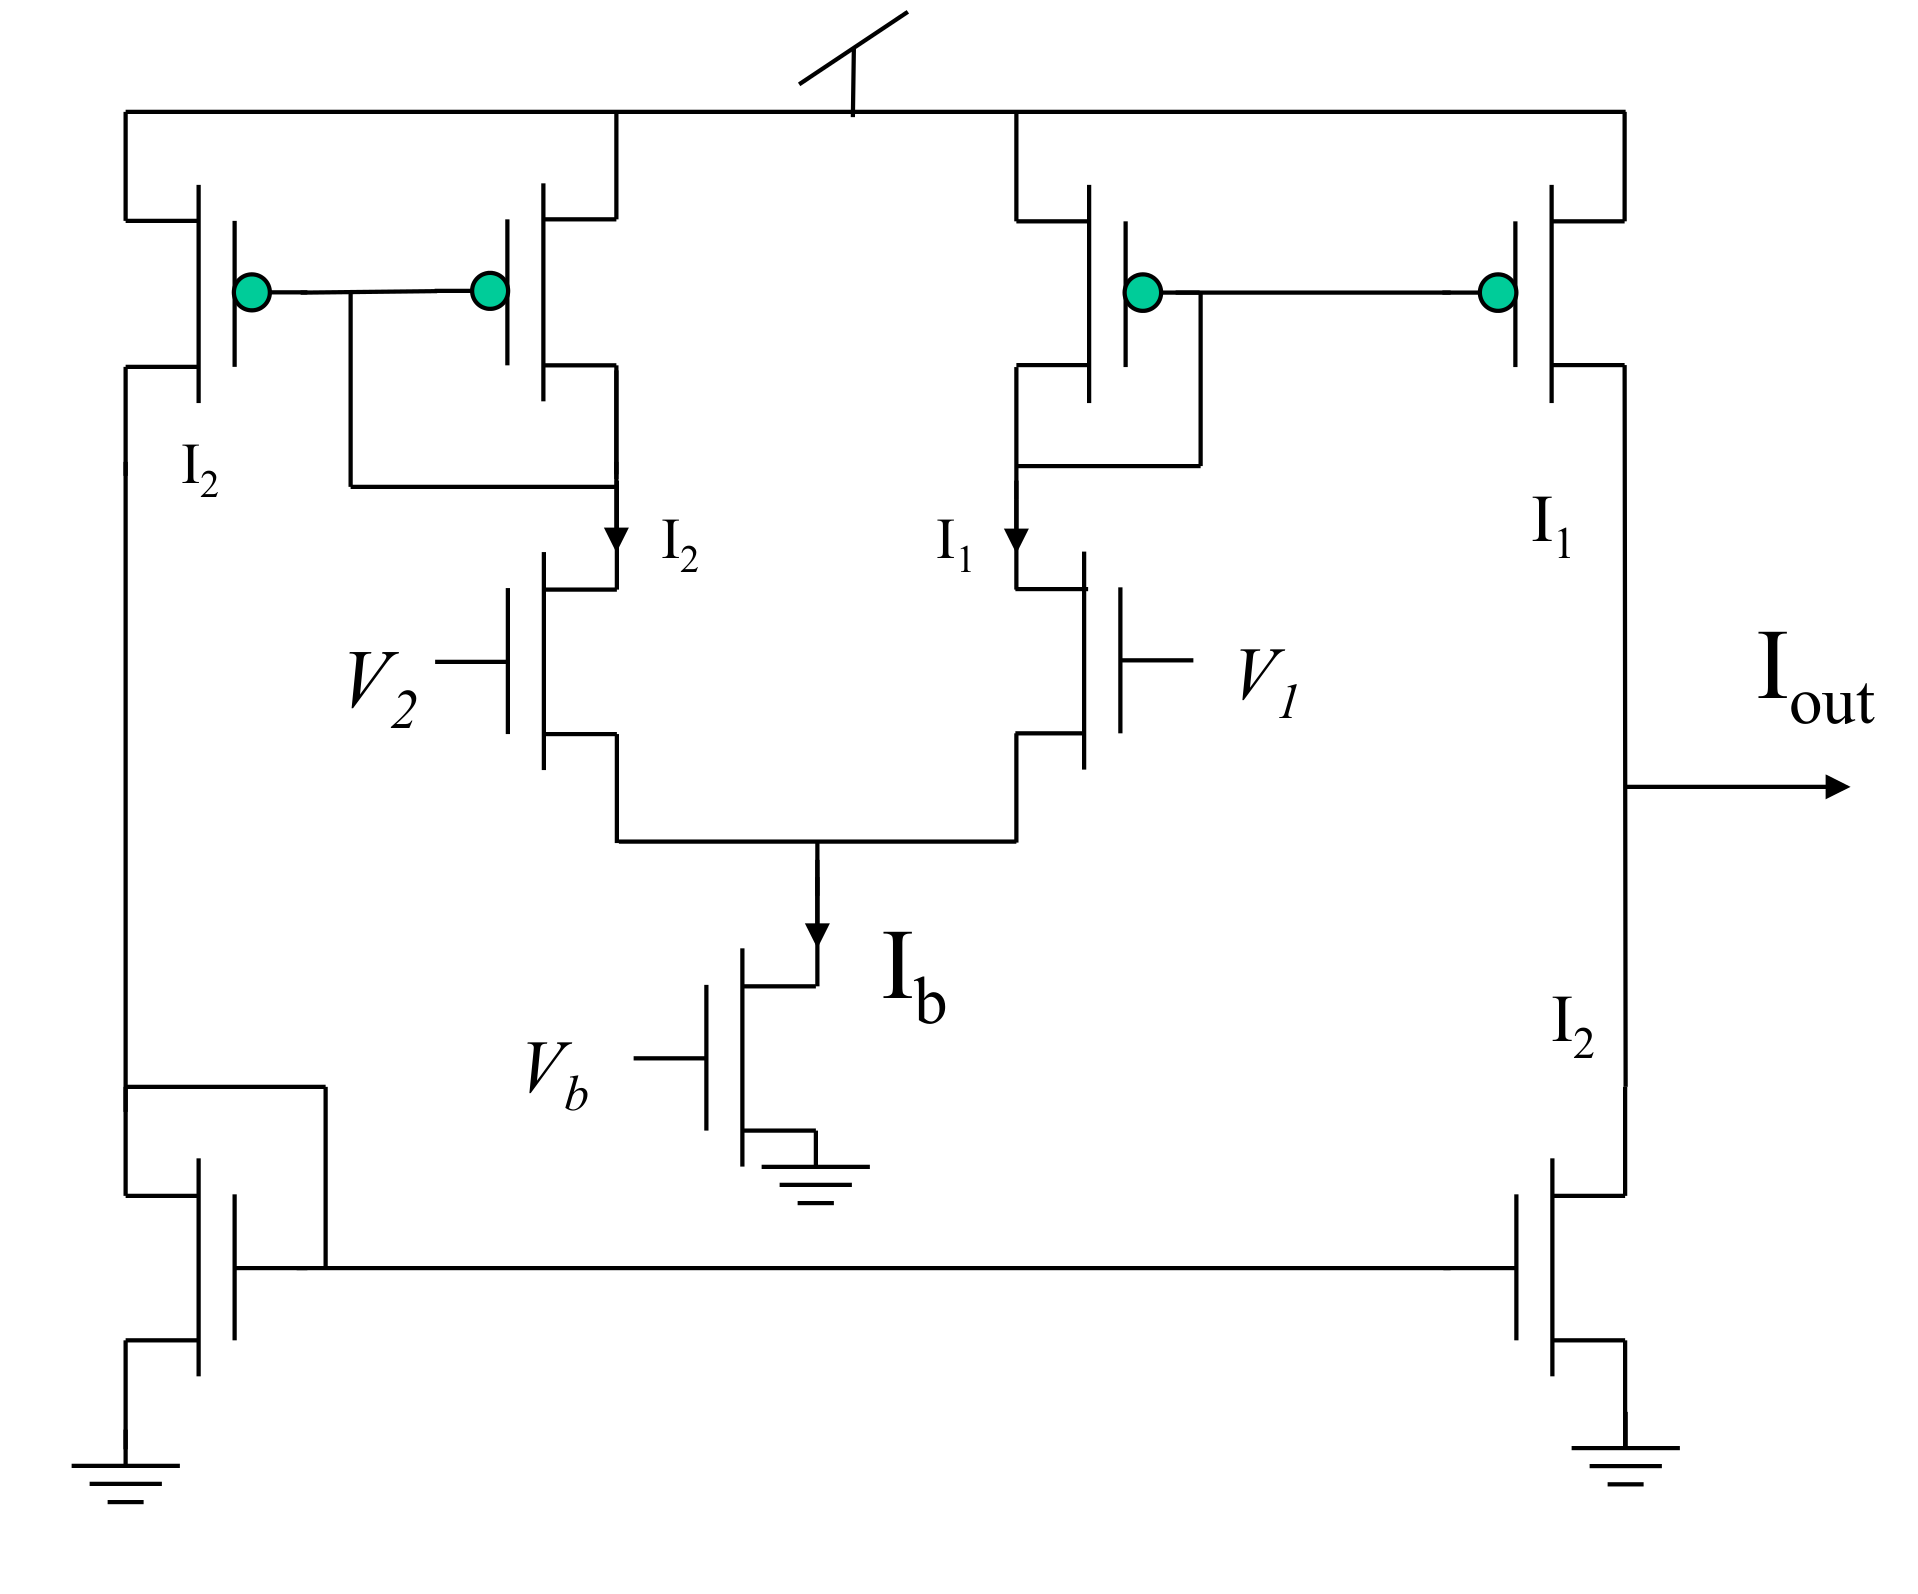
\includegraphics[scale=0.5]{pics/wide_range_transamp.png}
  \caption{Wide Range Transconductance Amplifier \cite{lec4}}
  \label{fig:wr_Transamp}
\end{figure}\bigskip


A wide-output range transconductance amplifier behaves very similar to a simple transconductance amplifier. Even though the circuit looks very complicated, it only consists of a differential pair and three current mirrors. The goal of these mirrors is to remove the restrictions on the output voltage of the amplifier.
\par Each branch of the differential pair is connected to a current mirror, but the currents $I_1$ and $I_2$ are still separated. After that, the same thing is done as in the simple transconductance amplifier, where one current (in Fig. \ref{fig:wr_Transamp} this would be $I_2$) is mirrored to the same node as the other one, and this node is connected to the output of the amplifier. The differential pair is now no longer connected to the output, which removes its restrictions from the allowed output condition. The new condition is
$$ 4U_T < V_{out} < V_{dd} -4U_T$$.



\section{Current Divider}
% Joachim
\begin{figure}[htbp]
  \centering
  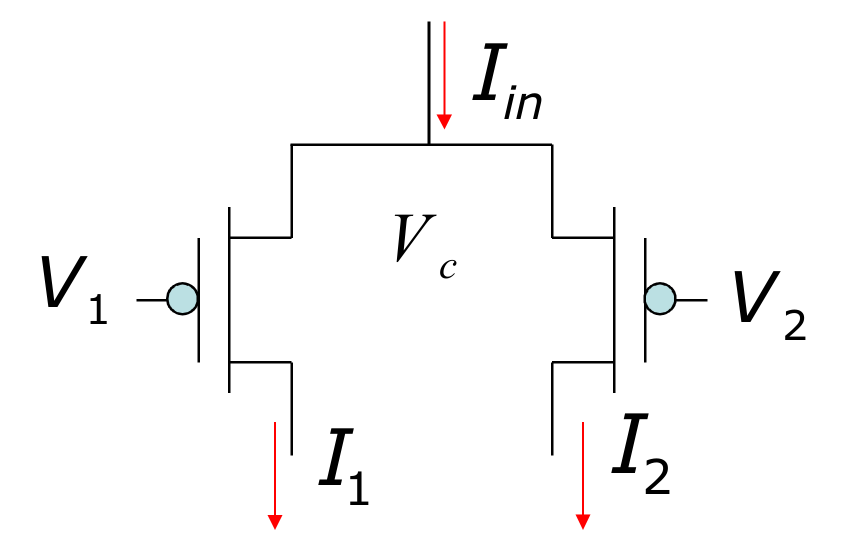
\includegraphics[scale=0.8]{pics/current_divider.png}
  \caption{Current Divider \cite{lec6}}
  \label{fig:current_divider}
\end{figure} 









% Dora Start

\section{Winner-take-all circuit (WTA)}
\subsection{How does the WTA circuit work?}

The circuit of Fig. \ref{fig:WTA} is a continuous time, analog circuit that implements
a WTA network, designed by Lazzaro et al. (1989).

It processes all the (continuous-time) input signals in
parallel, using only two transistors per input cell, and one global transistor
that is common to all cells. Collective computation and global connectivity is
obtained using one single node common to all cells.

\begin{figure}[htbp]
  \centering
  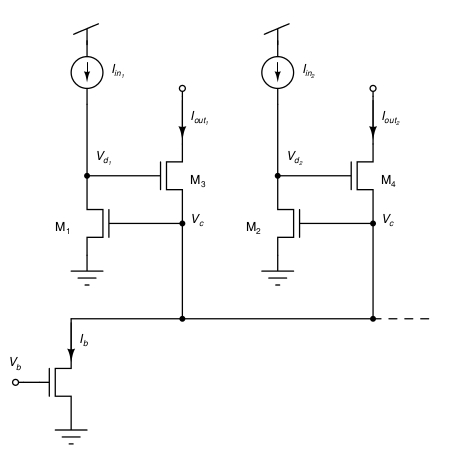
\includegraphics[scale=0.8]{pics/WTA.jpg}
  \caption{Two cells of a current mode WTA circuit \cite{book:VLSI}.}
  \label{fig:WTA}
\end{figure} 

The WTA network is modular and can be extended to n cells. 

Each cell comprises a current-controlled conveyor as in figure \ref{fig:current_conveyor}. The inputs of the circuit are applied currents,
output signals are encoded both by $I_{out}$ currents, and the $V_d$ voltages. 

\begin{figure}[htbp]
  \centering
  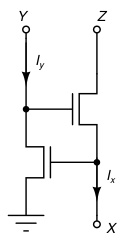
\includegraphics[scale=0.8]{pics/current_conveyor.jpg}
  \caption{Current-controlled conveyor \cite{book:VLSI}.}
  \label{fig:current_conveyor}
\end{figure} 

The application -- current coping in which the current-conveyor circuit is used in WTA is showed in the figure \ref{fig:current_conveyor_application}. Before to copy a current we used the current-mirror. It is very efficient -- as we need 1 transistor less. However, as the output of the circuit is connected in feed-back loop to the input, the sum of parasitic capacitances $C_{gs}$ will significantly slow down the output. In the most drastic case the outputs will even not detect any change in input current signal -- for high frequency time variant inputs (slew-rates limites output respond, higher time constant $\tau = RC$).

\begin{figure}[htbp]
  \centering
  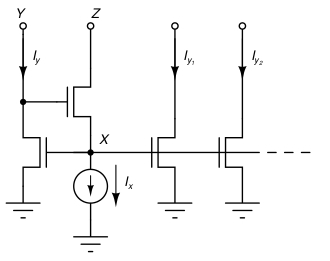
\includegraphics[scale=0.8]{pics/current_conveyor_application.jpg}
  \caption{System application of current conveyor for the generation of multiple copies of an input current \cite{book:VLSI}.}
  \label{fig:current_conveyor_application}
\end{figure} 

Transistors $M_1$ and $M_2$ discharge nodes $V_d$ -- implement inhibitory feedback. Transistors $M_3$ and $M_4$
 implement an excitatory feed-forward path by charging node $V_c$ . 
 
 The circuit selects the largest input current because cell provides j provides $I_{out}^j = I_b$  and so suppresses all other output voltages and currents (all other $V_d \approx 0$ and $I_{out} \approx 0$). Cell j wins the competition because its voltage $V_d^j$
determines $V_c$ ($V_{gs}$ is set by fixed value of $I_b$). Since all cells have common $V_c$ gate potentials it will be grater than $V_d$ for all other cells than j -- they will be shut-off \cite{book:VLSI}. 




\textit{Briefly: the circuit chooses one winner by selecting a cell with the highest input current (max() function). All other cells are suppressed (inhibited).}

Hysteretic WTA: by feeding back the output of the circuit to its input, the system gets more stable and less sensitive to probable new winner.

\subsection{Can you reason through its behaviour?}
We consider three cases (the network with two cells): 

\begin{enumerate}[label={I.}]
\item inputs are equal; 
\item one input much larger than the other; 
\item two inputs differ by a very small amount (small-signal regime).
\end{enumerate}

\begin{enumerate}[label={I.}]
\item Because gates of $M_1$ and $M_2$ are tied to the same common node $V_c$, the drain voltages of $M_1$ and $M_2$ must take the same value. As a result, the output transistors $M_3$ and $M_4$ will have equal $V_{gs}$ value and in case both of them are in saturation, the output currents have to be identical. Upon Kirchhoff's current law:
\begin{equation}
I_{out_1} = I_{out_2} = \frac{I_b}{2} 
\end{equation}

\item 

We can consider the case in which $I_{in_1}\gg I_{in_2}$. In this case, the drain voltage of $M_1$ ($V_{d_1}$) will be greater than the drain voltage of $M_2$ ($V_{d_2}$).

Because the two transistors $M_1$ and $M_2$ have a common gate voltage $V_c$, and both their sources are tied to ground, the froward current (dependent only on $V_{gs}$) for both them is equal. The need to suppress the value of forward current through $M_2$ arises. Therefore voltage $V_{d_2}$ has to be decreased (lower current for the same gate-to-source voltage ). We say that reverse current -- dependent only on $V_{ds}$ -- will increase, limiting overall current through drain to $I_{in_2}$ value. 

Decrease of $V_{d_2}$ causing $M_2$ to operate in its ohmic region (out of saturation), switches off $M_4$. This implies $I_{out_2}=0$. 

Consequently, output transistor $M_3$ sources all the bias current 
\begin{equation}
I_{out_1} = I_b,
\end{equation}
with $V_{d_1}$ satisfying the equation 
\begin{equation}
I_0 e^{\kappa V_{d_1}- V_c} = I_b.
\end{equation}

\item 
To analyze the circuit in this regime, we will use small-signal analysis. We must consider the Early effect of the transistor operating in the saturation region (Eq. \ref{eq:WTA_early_effect}):

\begin{equation}
I_{ds} = I_{sat}(1+ \frac{V_{ds}}{V_e})
\label{eq:WTA_early_effect}
\end{equation}
, $V_e$ is the Early voltage.
By derivating this equation (small-signal analysis) we get: $\delta I_{ds} = I_{sat} \frac{\delta V_{ds}}{V_e})$.

Assume that the two input currents $I_{in_1}$ and $I_{in_2}$ are initially equal. 

If we now increase the input current $I_{in_1}$ by a small amount $\delta I$ we would like to be able to obtain a difference in $M_1$ transistor's $V_{d_1}$, which is:
\begin{equation}
\delta V_d = \delta I_d \frac{V_e}{I_{sat}}
\end{equation}

As $V_{d_1}$ is also the gate voltage of transistor $M_3$, the $I_{out_1}$ will be amplified by an amount proportional to $e^{\delta V}$ . The Kirchhoff's law requires that
$I_{out_2}$ decreases by the same amount. This reduction means the gate voltage $V_{d_2}$ of $M_2$ must decrease by $\delta V$ \cite{book:VLSI}.
\end{enumerate}

All three cases can be summarised by the graphic \ref{fig:WTA_response}.

\begin{figure}[htbp]
  \centering
  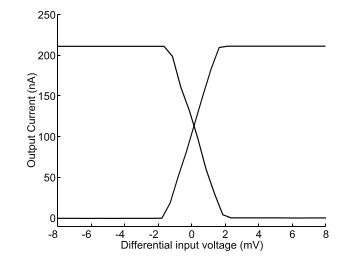
\includegraphics[scale=0.9]{pics/WTA_response.jpg}
  \caption{Responses of the two-cell WTA circuit. Current output ($I_{out_1}$ and $I_{out_2}$). The bias voltage $V_b = 0.7V$ \cite{book:VLSI}.}
  \label{fig:WTA_response}
\end{figure} 

\subsection{How does the bias current affect its performance?}
With increasing bias current it will get harder to choose a winner -- it takes larger input current difference to suppress all cells excluding the winner. 

???
\subsection{How can you adjust the gain of the circuit by layout of the transistors?}
Since the gain in the small-signal regime of the competition of the WTA circuit is expressed by equation:
\begin{equation}
\frac{\delta V}{\delta I} = \frac{V_e}{I_{sat}} 
\end{equation}
the only transistors' layout variables are early Voltage $V_e$ (dependent on the length of transistor) and $I_0$ coefficient of the saturation current (linearly dependent on $W/L$). Therefore, we can increase the gain by decreasing the width of the transistor or by increasing its length. 

???


\section{Photodiodes, photoreceptor}

\subsection{How does the I-V curve of a diode change in the presence of light?}

The current-voltage characteristic of a photodiode has the same
shape as that of a normal diode, but the curve is displaced along the current
axis by the value of the photocurrent (see fig. \ref{fig:photodiode_charac}).

\begin{figure}[htbp]
  \centering
  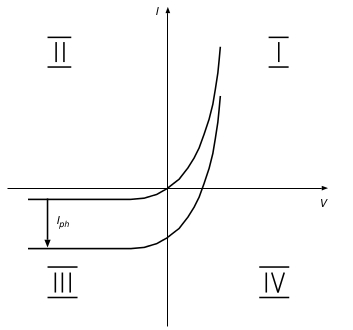
\includegraphics[scale=0.8]{pics/photodiode_charac.jpg}
  \caption{Steady-state current-voltage characteristics of a photodiode. The upper curve is the normal diode characteristic (dark characteristic). The lower curve shows the characteristic under illumination \cite{book:VLSI}.}
  \label{fig:photodiode_charac}
\end{figure} 

In the presence of an applied external bias the (negative) photocurrent  is superimposed onto the diode current.

\subsection{How does phototransduction occur in silicon?}

Transduction means transformation of the energy from one form to another. Phototransduction means transforming from photon to electronic signals \cite{lab8}.

In a semiconductor, an incident photon and therefore its energy can be absorbed by an electron. A
photon with an energy larger than or approximately equal to the bandgap energy can excite an electron from the valence band into the conduction band
(corresponds to the generation of an electron-hole pair). Illumination of a semiconductor therefore increases the concentration of mobile charge carriers (electrons). 

If the motion of the carriers is driven by diffusion, then the
generation is balanced by recombination(creation of pairs).

However, if electron-hole pairs are generated in depletion region and subjected to its built-in electric field, pairs are likely to be separated.  
Some of the separated carriers contribute to an electrical output signal (reverse photo current). The separated mobile charges are "swept home" as the minority charges dominate in depletion region. 

\begin{figure}[htbp]
  \centering
  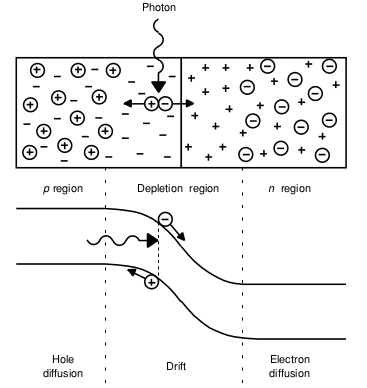
\includegraphics[scale=0.8]{pics/photodiode_principle.jpg}
  \caption{Principle of operation of a photodiode. Electron-hole pairs generated by incident photons in or
within a diffusion length outside the depletion region become separated and contribute to a reverse
generation current \cite{book:VLSI}.}
  \label{fig:photodiode_principle}
\end{figure} 

If the photodiode is open-circuited, that is, no external current is allowed
to flow, then generated charge accumulates at the boundaries of the depletion
region until a steady state is attained. In steady state, a forward diffusion current in
the junction compensates for the photo-
current \cite{paper:photo}.

If the photodiode terminals are short-circuited the photocurrent
can be measured as a reverse diode current. In the presence of an applied ex-
ternal bias the photocurrent is superimposed onto the diode current \cite{book:VLSI}.



\subsection{How you can use adaptation in a feedback loop to cancel out circuit mismatch?}

In the simple source-follower logarithmic photoreceptor circuit (see fig. \ref{fig:photoreceptor_log}) in real world application there are two important problems: mismatches and slow response (because the the huge capacitance have to be charged and discharged -- photodiode junction $C$ and the parasitic $C_{ds}, C_{gs}$, by a very small photocurrent). 

\begin{figure}[htbp]
  \centering
  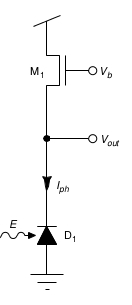
\includegraphics[scale=0.8]{pics/photoreceptor_log.jpg}
  \caption{Photosensors with logarithmic irradiance-to-voltage conversion consisting of a photodiode and a MOSFET in source-follower configuration \cite{book:VLSI}.}
  \label{fig:photoreceptor_log}
\end{figure} 

The differences between supposedly identical receptor outputs are as large as the typical signals
variations produced by real scenes -- circuit is unusable. Hence the necessity for adaptation in a feedback loop, to deal with the circuit mismatch problem (see fig. \ref{fig:photoreceptor_adaptive}).


\begin{figure}[htbp]
  \centering
  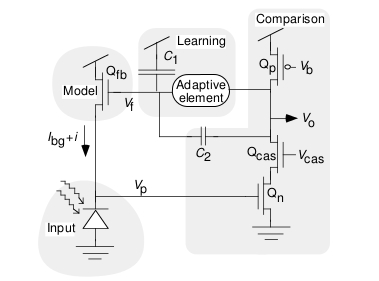
\includegraphics[scale=0.8]{pics/photoreceptor_adaptive.jpg}
  \caption{Adaptive receptor circuit \cite{paper:photo}.}
  \label{fig:photoreceptor_adaptive}
\end{figure} 

\textit{Briefly: The feedback amplifier and the input fight to control the source voltage of $Q_{fb}$, but the feedback amplifier wins because it has much higher gain. The input voltage $v_p$ moves enough so that the output voltage $v_o$ moves enough so that $v_f$ moves enough so that $v_p$ is held nearly clamped. }

The photocurrents are proportional to the areas of the corresponding photodiode junctions, whose spatial variations are the main source
of photocurrent mismatches of identically designed photosensing elements resulting in \textit{fixed-pattern noise}.

The FPN can be reduced by individual tuning of each photosensor. A more economic solution is the enhancement
of transient signals with respect to the mismatched steady-state signals using a
well-matched amplifier stage (capacitive-devider). Adaptation to the DC value can be provided by a resistive element \cite{book:VLSI}.

Adaptive element (see fig. \ref{fig:photo_adaptive_element_schematic}) has current-voltage relationship as shown in the fig. \ref{fig:photo_adaptive_element}.

\begin{figure}[htbp]
\centering
  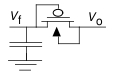
\includegraphics[scale=0.8]{pics/photo_adaptive_element_schematic.jpg}
  \caption{Expansive adaptive element with the capacitor that stores the adaptation state \cite{paper:photo}.}
  \label{fig:photo_adaptive_element_schematic}
\end{figure} 

\begin{figure}[htbp]
  \centering
  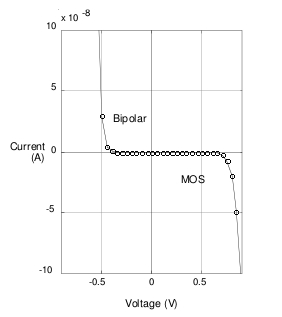
\includegraphics[scale=0.8]{pics/photo_adaptive_element.jpg}
  \caption{Measured current–voltage relationship for the adaptive element. The voltage scale changes logarithmically with the current scale \cite{paper:photo}.}
  \label{fig:photo_adaptive_element}
\end{figure} 


Due to the use of an adaptive element with an expansive nonlinearity there is different respond to input:

\begin{itemize}
\item Large changes (high frequencies, huge changes in illumination, ambient lighting, background change -- from shadow into sunlight) adapt rapidly.  Low gain for static signals (including circuit mismatches) --  the feedback is a short circuit across the adaptive element.
%, and $v_o$ does not need to move much to hold $v_p$ clamped. ??????????????????????????????????????????????????only once instead back of back and forth
\item Small signals around an adaptation point (small contrast variation) adapt slowly. The transient gain of the receptor is high, set by the capacitive-divider ratio as no charge flows through the adaptive element, changes in $v_o$ are coupled to $v_f$ through the capacitive divider \cite{paper:photo}.
\end{itemize}

The amplitude of the response to the
small contrast variation is almost invariant
to the absolute intensity (as in retina in eye), owing to the logarithmic response property. 



\subsection{How you can build a fast logarithmic current-sense amplifier, by using feedback to make a virtual ground?}

To make a virtual ground -- to clamp voltage $V_s$ to constant level.

 $V_s$ node is output of the source-follower log receptor with high parasitic capacitance -- requiring a lot of time to charge or discharge it -- circuit is not responding to high frequencies.  By decoupling output node from the $V_s$ node we get higher bandwidth (grater passband of frequencies).
Hence the necessity for active feedback, to deal with the problem of slow response  \cite{paper:photo}. For the circuit schematic see fig. \ref{fig:photosensor_feedback}

\begin{figure}[htbp]
  \centering
  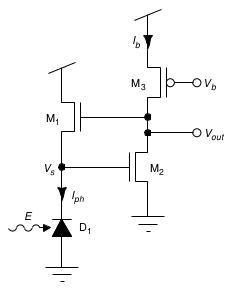
\includegraphics[scale=0.8]{pics/photosensor_feedback.jpg}
  \caption{Logarithmic photosensor with feedback loop icreasing the bandwidth by clamping the voltage $V_s$ \cite{paper:photo}.}
  \label{fig:photosensor_feedback}
\end{figure} 

The voltage output signal then appears at the gate of the MOSFET $M_1$, while the source and therefore the
voltage across the photodiode is practically clamped. The source node drives $V_s$ a two-transistor inverting amplifier
with a pFET current source clamping $V_s$ \cite{book:VLSI}. 

\subsection{How you can use a capacitive divider in the feedback loop of an amplifier to set gain?}

The mismatches can be reduced by a well-matched transient gain stage fabricated with a capacitive divider.

On short time scales , no charge flows through the adaptive element, but changes in $v_o$ are coupled to $v_f$ through the capacitive divider (see fig. \ref{fig:photoreceptor_adaptive}). The transient gain of the receptor is thus set by the capacitive-divider ratio. 
\begin{equation}
A_c = \frac{C_1+C_2}{C_2}, ~~~ \delta V_{out}=A_c A \delta V_s
\end{equation}
The larger $C_1$ is relative to $C_2$, the larger the gain of the circuit \cite{book:VLSI}.

\subsection{How you can use a cascode configuration to increase effective drain resistance?}

If we take a cascode with 2 nFET transistors and name the upper one $M_c$ and the lower one $M_2$ and take variables $g_{dc}, g_{sc}$ -- drain and source, output, input transconductance of $M_c$, $g_{d2}$ -- drain, output transcondunctance of $M_2$ and $g_0$ -- overall conductance of the cascode, $V_x$ -- common node between 2 transistors we can write:
\begin{equation}
g_0 = \frac{\delta}{V_0},
\end{equation}
\begin{equation}
\delta = g_0 V_0 = g_{d2} V_0 - g_{sc} V_x,
\end{equation}
\begin{equation}
( g_{d2} + g_{sc} )V_x = g_{dc} V_0.
\end{equation}

Excluding unknown $V_x$ from both equation we get:
\begin{equation}
\delta = \frac{g_{d2} g_{dc} }{g_{d2} + g_{sc} } V_0 \approx  \frac{g_{d2} g_{dc} }{g_{d2} + g_{sc} } V_0.
\end{equation}
\begin{equation}
g_{0} = g_{d2} \frac{g_{dc}}{g_{sc}} \approx g_{d2} \frac{U_{T}}{V_{e}}.
\end{equation}

And finally we can derive the expression for the change resistance after connecting additional transistor in cascode configuration:
\begin{equation}
r_{0} = r_{d2} \frac{V_{e}}{U_{T}}.
\end{equation}
As we can see, the resistance will be increased by approximately $\frac{V_e}{U_T} \gg 1$.

\subsection{What is the Miller effect?}

The Miller effect occurs when a capacitor feeds back the output of an inverting, high gain amplifier back to the input. If the input needs to move a certain amount, it must charge not only its own side of the capacitor, but also the other side of the capacitor which moves $A$ times as much in the opposite direction. Hence a small capacitance $C$ looks like a capacitance $(A+1)C$ to the input. Since $A \gg 1$, we usually ignore the $1$. The Miller capacitors $C_n$  (see fig. \ref{fig:photoreceptor_adaptive}) from the gate to the drain of $Q_n$ has a substantial effect on the time-response of the receptor. The Miller effect increases the relevant gate–drain and gate–source capacitances by a factor of A  \cite{paper:photo}.

\subsection{How can a cascode be used to reduce it?}

The parasitic capacitance $C_p$ from the source of $M_1$ onto the output node via the gate-to-drain capacitance of nFET $M_2$ gives rise to the Miller effect (see fig. \ref{fig:photosensor_cascode}).

\begin{figure}[htbp]
  \centering
  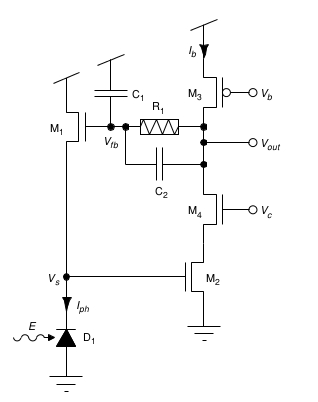
\includegraphics[scale=0.8]{pics/photosensor_cascode.jpg}
  \caption{Adaptive logarithmic photosensor with cascode transistor increasing the bandwidth for small photocurrents \cite{book:VLSI}.}
  \label{fig:photosensor_cascode}
\end{figure} 

Hereby, the apparent capacitance, as seen from the source of $M_1$ , is increased by $C_p$ multiplied by the voltage gain from gate to source. For small photocurrents this effect leads to limited response band width ($I = C \frac{\delta V}{dt}$). The introduction of a cascode with a fixed gate voltage $V_c$ clamps the voltage on the drain of $M_2$, because the current through the amplifier is approximately constant, and largely nullifies the Miller effect (parasitic capacitance has only influence on feedback for changing voltage). 

However, for certain biasing conditions the presence of the cascode can make the circuit unstable \cite{book:VLSI}.

\section{Silicon Neurons}
\subsection{What is a neuron and what are its components?}
The basic anatomical unit in the nervous system is specialised cell called the neuron.

\cite{book:Mead}

\begin{enumerate}
\item Synapse
\item Soma
\item Dendrite
\end{enumerate}
\subsection{What types of models are used to simulate neurons?}
\subsection{How does the spikegeneratng mechanism work?}
\subsection{What is an FI curve?}
\subsection{Can you draw the circuit schematic of the axon-hillock neuron?}
The schematic of the axon-hillock neuron can vary upon the chosen amplification. General schematic is depicted on the figure \ref{fig:neuron_hillock_general}.

\begin{figure}[htbp]
  \centering
  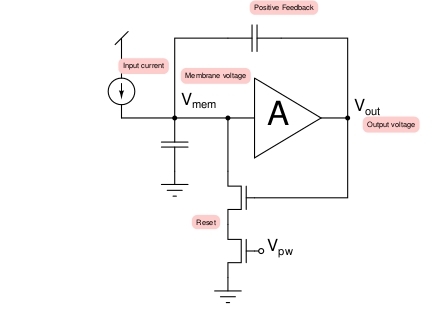
\includegraphics[scale=0.8]{pics/neuron_hillock_general.jpg}
  \caption{The Axon-Hillock circuit \cite{lecture11}.}
  \label{fig:neuron_hillock_general}
\end{figure} 

The specific amplification was chosen and is depicted on the Axon-hillock integrate and fire circuit (see fig. \ref{fig:neuron_hillock}).

\begin{figure}[htbp]
  \centering
  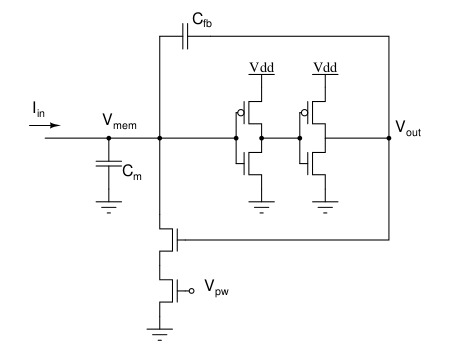
\includegraphics[scale=0.8]{pics/neuron_hillock.jpg}
  \caption{Axon-hillock integrate and fire circuit \cite{lab11}.}
  \label{fig:neuron_hillock}
\end{figure} 


\cite{lab11}.

\section{Important Values to Remember}

\subsection{Subthreshold slope factor $\kappa$}
nFET: 0.4- 0.9\\
pFET: 1

\subsection{Threshold Voltage $V_t$}
Typical value nFETs: 0.7V

\subsection{Early Voltage}
20-30V

\subsection{Dark Current}
? pico Amps?

\subsection{$I_0$}
nFET: $1\cdot10^{-14}$ A\\
pFET: $1\cdot10^{-18}$ A


\section{Exam Questions}
\begin{itemize}
\item Draw an argue through a photodiode
\item Explain the time domain ($\tau = R\cdot C$) of a photo diode
\item Draw and argue through a photodiode circuit with feedback and cascode
\item Draw and argue through a WTA circuit given all is in subthreshold, and $I_2$ current is bigger than $I_1$
\subitem Given current source 1 has voltage x, current source 2 has voltage y, and the bias voltage is z, what are the voltages of all the nodes in the circuit
\item What is $U_T$ and what does it stand for (Knowing the formula $U_T=\frac{kT}{q}$ is NOT enough! What does it physically mean?)
\end{itemize}


\section{Lab Questions}
\subsection{Lab 1}
\begin{itemize}
\item Remember: Experimental techniques and devices are never ideal.
\end{itemize}

\subsection{Lab 2}
\begin{itemize}
\item What does it mean for a MOS transistor channel to be accumulated, flat-band, depleted,
inverted? \item Knowledge of how subthreshold transistor operation is a diffusion process and
why it depends exponentially on the terminal voltages. \item What is the meaning of ”saturation”?
\item What is the triode or linear operating range? $I_{ds}$ vs $V_{gs}$ on log scale. \item Differences between
n- and p-fets. \item Typical values of $I_0$, $\kappa$ and subthreshold operating range. \item What are wells and how should the wells be biased relative to the substrate? \item What is the ”back gate” or ”body
effect”? \item How is the back gate is related to $\kappa$? \item How do you measure $\kappa$? \item How to make a
MOS capacitor and what is its C-V relationship. \item How a source follower works and how to
compute the gain of a source follower.
\end{itemize}

\subsection{Lab 3}
\begin{itemize}
\item How transistors work above threshold. \item What is the linear or triode region and what is the
saturation region? \item How they depend on gate and threshold voltage. What is the “over-
drive”? \item What is the specific current? How the Early effect comes about. \item Typical values for
Early voltage. \item How to sketch graphs of transistor current vs. gate voltage and drain-source
voltage. \item How above-threshold transistors go into saturation and why the saturation voltage
is equal to the gate overdrive. \item The above-threshold current equations. \item How above-threshold
current depends on Cox and mobility.
\item How transconductance and drain resistance combine to generate voltage gain and what is
the intrinsic voltage gain of a transistor.
\item What effect does velocity saturation have on transistor operation, specifically, how does
it change the relation between saturation current and gate voltage? \item What is DIBL (drain
induced barrier lowering) and II (impact ionization)?
\item What is the dominant source of mismatch? \item How does transistor mismatch scale with tran-
sistor size? \item What are typical values of transistor threshold voltage mismatch?
\end{itemize}



\subsection{Lab 4}
\begin{itemize}
\item Can you sketch a transamp, a wide range transamp, a current correlator, and a bump circuit
in both n- and p-type varieties?
\item How does a differential pair work? \item How does the common-node voltage change with the
input voltages? \item How can you compute the differential tail currents from the subthreshold
equations, and how do you obtain the result in terms of the differential input voltage?
\item How does a current-correlator work? \item How does a bump circuit work?
\item The I-V characteristics of a transconductance amplifier below threshold. \item What’s the
functional difference between simple and wide-output-range transamp? \item The subthreshold
transconductance gm . \item The relation between gain A, transistor drain conductances gd , and
transconductances gm .
\item Can you reason through all the node voltages in these circuits? I.e., if we draw the circuit
and provide specific power supply and input voltages, can you reason to estimate all the
other node voltages, at least to first order approximations, assuming $\kappa$ = 1?
\end{itemize}



\subsection{Lab 6}
\begin{itemize}
\item How does the WTA circuit work? \item Can you reason through its behavior? \item How does the bias
current affect its performance? \item How can you adjust the gain of the circuit through the sizing
of the transistors?
\end{itemize}


\subsection{Lab 7}
\begin{itemize}
\item How to use an oscilloscope and a function generator. \item How to compute the time-constant of
a low-pass filter and how to estimate it from the measurements. \item  to change the time-
constant of a follower-integrator circuit. \item In what way does the follower integrator behave
nonlinearly for large signal input?
\end{itemize}


\subsection{Lab 8}
\begin{itemize}
\item How does the I-V curve of a diode change in the presence of light? \item How does phototrans-
duction occur in silicon?
\end{itemize}


\subsection{Lab 9}
\begin{itemize}
\item How you can use adaptation in a feedback loop to highpass amplify signal but not mismatch.
\item How you can build a fast logarithmic current-sense amplifier, by using feedback to make a
virtual ground. \item How you can use a capacitive divider in the feedback loop of an amplifier to
set a gain. \item How you can use a cascode configuration to increase effective drain resistance.
\item What is the Miller effect, and how a cascode can be used to nullify it.
\end{itemize}


\subsection{Lab 10}
\begin{itemize}
\item The schematic for a synapse circuit. \item How the synaptic current changes as a function of the
synaptic weight, the time constant, and the presynaptic frequency.Can
\end{itemize}


\subsection{Lab 11}
\begin{itemize}
\item What is a neuron and what are its components (synapse, soma, dendrite)? \item What types of
models are used to simulate neurons? \item How does the spike-generating mechanism work?
\item What is an FI curve? \item Can you draw the circuit schematic of the axon-hillock neuron?
\end{itemize}


\subsection{Lab 12}
%Joachim
\begin{itemize}
\item How do tunneling and injection mechanisms work? \item What is the shape of the energy band
diagram in the channel and oxide during tunneling and injection? \item How are the memory cell
circuits used to control tunneling and injection?
\end{itemize}

\section{TODO}
\begin{itemize}
\item \textbf{ADD THE EXAM QUESTIONS YOU GOT ASKED!!} (The guys next year will thank you!)
\item Improve layout (currently ugly at some points...)
\item Complete "Silicon Neurons" chapter
\item Complete current divider circuit
\item Add more values to "Important Values to Remember"
\item Add more basic theory (e.g. definition and meaning of $U_T$)
\end{itemize}

\newpage
\begin{thebibliography}{7}
\bibitem{book:VLSI}
Liu, Kramer, Delbrück, Indiveri, Douglas -- \emph{Analog VLSI: Circuits and Principles}, 2002 -- Massachusetts Institute of Technology
\bibitem{book:Mead}
Carver Mead -- \emph{Analog VLSI and Neural Systems}, 1989 -- Addison-Wesley Publishing Company
\bibitem{lecture11}
Delbrück, Indiveri, Liu -- \emph{Neuromorphic Engineering I, Fall Semester 2013, Silicon neurons. Integrate and fire models. Analog VLSI implementations of adaptive neurons. The silicon neuron: detailed VLSI model with adaptation properties. }
\bibitem{lab4}
Delbrück, Indiveri, Liu -- \emph{Neuromorphic Engineering I, Fall Semester 2013, Lab 4 Document}
\bibitem{lab8}
Delbrück, Indiveri, Liu -- \emph{Neuromorphic Engineering I, Fall Semester 2013, Lab 8 Document}
\bibitem{lab11}
Delbrück, Indiveri, Liu -- \emph{Neuromorphic Engineering I, Fall Semester 2013, Lab 11 Document}
\bibitem{lec2}
Delbrück, Indiveri, Liu -- \emph{Neuromorphic Engineering I, Fall Semester 2013, Lecture 2 Document}
\bibitem{lec4}
Delbrück, Indiveri, Liu -- \emph{Neuromorphic Engineering I, Fall Semester 2013, Lecture 4 Document}
\bibitem{lec6}
Delbrück, Indiveri, Liu -- \emph{Neuromorphic Engineering I, Fall Semester 2013, Lecture 6 Document}
\bibitem{paper:photo}
T. Delbrück, C.A. Mead -- \emph{Analog VLSI Phototrunsduction by continous-time, adaptive, logartihmic photoreceptor circuits}, CNS Memo no.30, April 2. 1996 -- California Institute of Technology
%\bibitem{handbook:hamamatsu} Hamamatsu Photonics K.K. -- \emph{Opto-semiconductor Handbook Chapter 2:Si photodiodes}
%\url {http://www.hamamatsu.com/resources/pdf/ssd/e02_handbook_si_photodiode.pdf}
%\bibitem{book:analog_CMOS}
%Phillip E. et al, -- \emph{CMOS Analog Circuit Design (The Oxford Series in Electrical and Computer Engineering), Third Edition}, 2011 -- Oxford University Press
%\bibitem{web:wikiUt}
%Boltzmann constant -- \url{http://en.wikipedia.org/wiki/Boltzmann_constant}
%\bibitem{paper:channelmodulation}
%K. Venkateswaren -- \emph{Effects of channel potential modulation in narrow channel CCD shift registers}, 1978 -- IEEE, Fairchild Semiconductor Palo %Alto, California
%\bibitem{paper:mulder}
%Mulder et. al. -- \emph{Application of the Back Gate in MOS Weak Inversion Translinear Circuits}, 1995 -- IEEE Transactions on Circuits and Systems, Vol. 42, Nr. 11
\end{thebibliography}